\chapter{Performance Evaluation}
\label{cha:result}
The filter has been evaluated in several different ways.
To get an idea if the filter structure is reasonably formulated or not, an initial observability analysis has been done.
If the filter structure, including the target modelling and measurement setups, is not plausible, a reformulation of the problem might be necessary.
Monte Carlo simulations were then used to obtain some statistical properties, and a theoretical performance analysis, without having to calculate it analytically.
Since the filter depends on the quality of the constructed angular rate measurements, the selected homography estimation method has been evaluated through simulations.

To see how the filter perform compared to a stereo camera system, two sequence were recorded and the output has been compared with the output from the filter constructed in this thesis.

\section{Observability along Different Trajectories}
\label{sec:observabilityresult}
In order to see if the filter structure is reasonably formulated, \ie if the target modelling and the measurement setups have been suitably chosen, an observability analysis according to \Sectionref{sec:observabilitymethod} has been performed and summarized in \Tableref{tab:observabilityresult}.
The results show that the filter is formulated such that a trajectory with a moving target seems to be observable.
A trajectory of a target with no ego motion is observable only if all three types of measurements are available.
It is not observable if only \abbrROI and angular rate measurements are available.

\begin{table}[!ht]
	\centering
	\caption{\label{tab:observabilityresult} A summary of the observability analysis results for different trajectories and different measurement setups.}
	\begin{tabular}{|p{5cm}|p{1cm}|p{2cm}|p{2.5cm}|}
		\cline{2-4}
		\multicolumn{1}{c|}{} & \multicolumn{3}{c|}{\textbf{Observable}} \\
		\hline
		\textbf{Description} & \abbrROI & \abbrROI and angular rate & \abbrROI, angular rate and corners \\
		\hline
		The target is standing still with an arbitrary initial yaw angle. & No & No & Yes \\
		\hline
		The target is driving straight towards or straight away from the host. & Yes & Yes & Yes \\
		\hline
		The target is driving towards or away from the host applying sine steering. & Yes & Yes & Yes \\
		\hline
		The target is driving away from the host and makes a $45^\circ$ turn. & Yes & Yes & Yes \\
		\hline
		The target is driving across the host's lane with constant speed and constant yaw angle. & Yes & Yes & Yes \\
		\hline
	\end{tabular}
\end{table}

A intuitive explanation to why that particular situation is not observable is that, if the target has no ego motion and only \abbrROI and angular rate are used as measurements, the same \abbrROI measurements could be observed from several different target state vectors.
For example could the same \abbrROI appear if the target is rotated either $\pm\psi$ and the $(x,y,z)^T$ position is adjusted accordingly.
The \abbrROI will appear the same in the image plane.

Since it is difficult to prove general observability for nonlinear systems, these results at least gives a hint if the filtering problem is solvable or not.
The filter should, in the selected test cases where the target had an ego motion, be able to estimate the given trajectory.

\newpage

\section{Monte Carlo Simulations}
\label{sec:montecarloresult}
By first simulating the filter using the Monte Carlo method, a rough evaluation of the filter's performance can be obtained.
In Monte Carlo simulations, the available measurements and the measurement noise levels can be controlled.
It is always good to know what to strive for when running the filter on real-world data.
The goal of performing the Monte Carlo simulations is to get results about what qualities on the measurements that are required in order to get a good state estimate, especially regarding the angular rate measurements.

Two different scenarios were simulated, with different noise realisations.
The applied noise was Gaussian, with zero mean and different covariance matrices.
The covariance matrices $\bm{Q}^\text{sim}$ and $\bm{R}^\text{sim}$ were used when simulating the trajectory and generating the measurements while $\bm{Q}$ and $\bm{R}$ were used when estimating the trajectory.
The simulation covariance matrices were
\begin{align}
	\label{eq:Qsim}
	\bm{Q}^\text{sim} &=
	\begin{pmatrix}
		0 & 0 & 0 & 0 & 0 & 0 \\
		0 & 0 & 0 & 0 & 0 & 0 \\
		0 & 0 & 0 & 0 & 0 & 0 \\
		0 & 0 & 0 & 0.0001 & 0 & 0 \\
		0 & 0 & 0 & 0 & 0 & 0 \\
		0 & 0 & 0 & 0 & 0 & Q^\text{sim}_\omega
	\end{pmatrix}
	,
	\\
	\label{eq:Rsim}
	\bm{R}^\text{sim} &=
	\begin{pmatrix}
		10 & 0 & 0 & 0 & 0 & 0 \\
		0 & 10 & 0 & 0 & 0 & 0 \\
		0 & 0 & 10 & 0 & 0 & 0 \\
		0 & 0 & 0 & R^\text{sim}_\omega & 0 & 0 \\
		0 & 0 & 0 & 0 & 10 & 0 \\
		0 & 0 & 0 & 0 & 0 & 10
	\end{pmatrix}
	.
\end{align}
The $\bm{Q}$ and $\bm{R}$ matrices were tuned in order to get good state estimates.
The initial state, $\bm{x}_0$, of the target was set to
%
\begin{equation*}
	\bm{x}_0 =
	\begin{pmatrix}
		p_\text{Bottom} & p_\text{HCP} & -1.5 & 0 & 0 & 0
	\end{pmatrix}^T.
\end{equation*}
%
Here, $p_\text{Bottom}$ and $p_\text{HCP}$ means that the measurement equations for the \abbrROI bottom and \abbrROI horizontal center position were used to initialize the $x$ and $y$ states, respectively.

\newpage

First, a simulation of a target detected 15 meters in front of the host, driving straight away with a constant velocity of 5 m/s, was evaluated.
The used measurements and the parameters $Q^\text{sim}_\omega$ and $R^\text{sim}_\omega$ varied according to \Tableref{tab:montesimscenario1}.
%
\begin{table}[!ht]
	\centering
	\caption{\label{tab:montesimscenario1} The simulation parameters and available measurements for different setup cases of the first simulated scenario.}
	\renewcommand{\arraystretch}{1.2}
	\begin{tabular}{|l|p{3.5cm}|l|l|}
		\hline
		\textbf{Setup no.} & \textbf{Measurements} & $Q^\text{sim}_\omega$ (rad/s) & $R^\text{sim}_\omega$ (rad/s) \\
		\hline
		1 & \abbrROI & $1.7\cdot 10^{-6}$ & -- \\
		\hline
		2 & \abbrROI and angular rate & $1.7\cdot 10^{-6}$ & 0.1 \\
		\hline
		3 & \abbrROI and angular rate & $1.7\cdot 10^{-6}$ & 0.5 \\
		\hline
		4 & \abbrROI and angular rate & $1.7\cdot 10^{-6}$ & 1 \\
		\hline
		5 & \abbrROI, angular rate and corners & $1.7\cdot 10^{-6}$ & 0.1 \\
		\hline
	\end{tabular}
\end{table}

In this scenario, the covariance matrices $\bm{Q}$ and $\bm{R}$ were
\begin{align}
	\label{eq:Qsim1}
	\bm{Q} &=
	\begin{pmatrix}
		0.25 & 0 & 0 & 0 & 0 & 0 \\
		0 & 0.1 & 0 & 0 & 0 & 0 \\
		0 & 0 & 0.05 & 0 & 0 & 0 \\
		0 & 0 & 0 & 1 & 0 & 0 \\
		0 & 0 & 0 & 0 & 0.00017 & 0 \\
		0 & 0 & 0 & 0 & 0 & 0.0017 \\
	\end{pmatrix}, \\
	\label{eq:Rsim1}
	\bm{R} &= 10 \bm{R}^\text{sim},
\end{align}
in all setup cases.
The matrix $\bm{R}^\text{sim}$ is given by \eqref{eq:Rsim}.

The results for each setup can be seen in \Figuresref{fig:27montesimstraighttowardsroirmse}--\ref{fig:30montesimstraighttowardsroiangvelcornerrmse}.
Examples of the simulated trajectories can be found in \Figuresref{fig:27montesimstraighttowardsroitrajpos}--\ref{fig:30montesimstraighttowardsroiangvelcornertrajother} in \Appendixref{app:montecarlo}.

If only \abbrROI measurements were used, the filter performed poorly as can be seen in \Figureref{fig:27montesimstraighttowardsroirmse}.
Especially with regard to the orientation, \ie the yaw angle.
If additionally to the \abbrROI measurements, angular rate measurements were added, a significant improvement were obtained, as can be seen in \Figureref{fig:20montesimstraighttowardsroiangvelrmse}.
Here, the noise variance level were 0.1 rad/s.
In \Figuresref{fig:21montesimstraighttowardsroiangvelrmse} and \ref{fig:22montesimstraighttowardsroiangvelrmse}, the \abbrRMSE of the estimated states diverged quickly due to the high noise level of the angular rate measurements.
The noise variance levels were 0.5 rad/s and 1 rad/s, respectively.
Note especially the difference in the yaw angle comparing \Figureref{fig:20montesimstraighttowardsroiangvelrmse} to \Figuresref{fig:21montesimstraighttowardsroiangvelrmse} and \ref{fig:22montesimstraighttowardsroiangvelrmse}.
The idea of adding the measurements of the target's corners, considering \Figureref{fig:30montesimstraighttowardsroiangvelcornerrmse}, resulted in an excellent state estimate.

\begin{figure}[!ht]
	\centering
	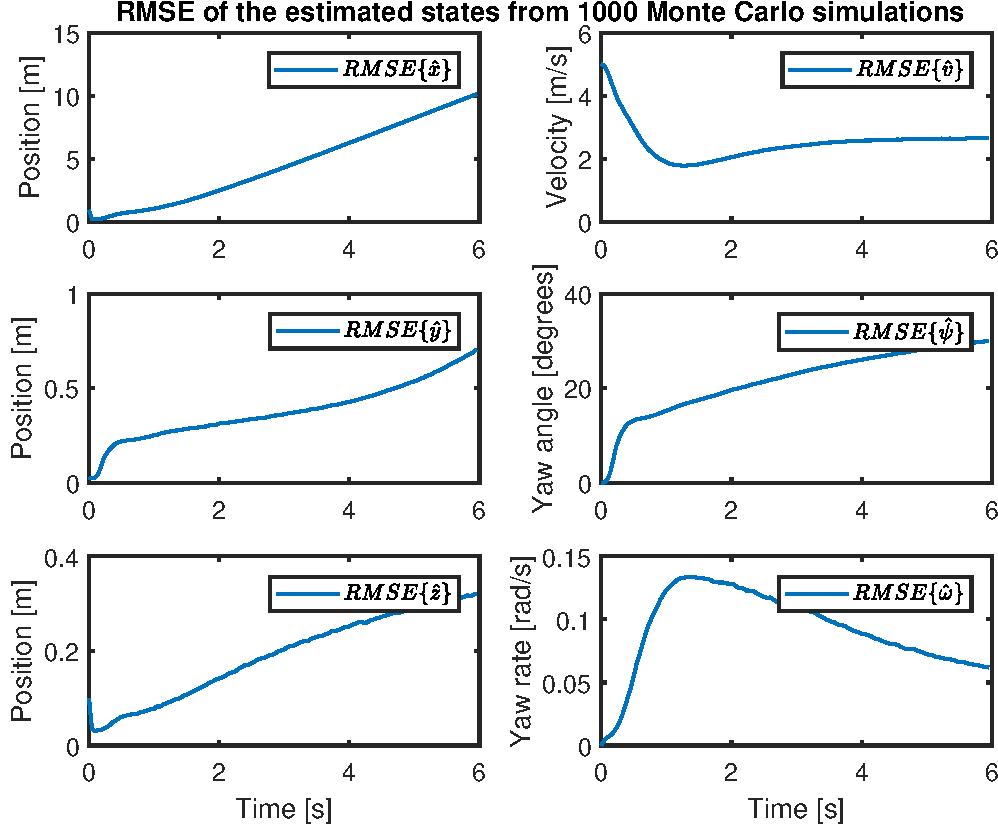
\includegraphics[width=0.8\textwidth]{MonteCarloSim/27_MC_1000_Rmse}
	\caption{\label{fig:27montesimstraighttowardsroirmse} Monte Carlo simulation result of scenario 1 with setup 1.}
\end{figure}

\begin{figure}[!ht]
	\centering
	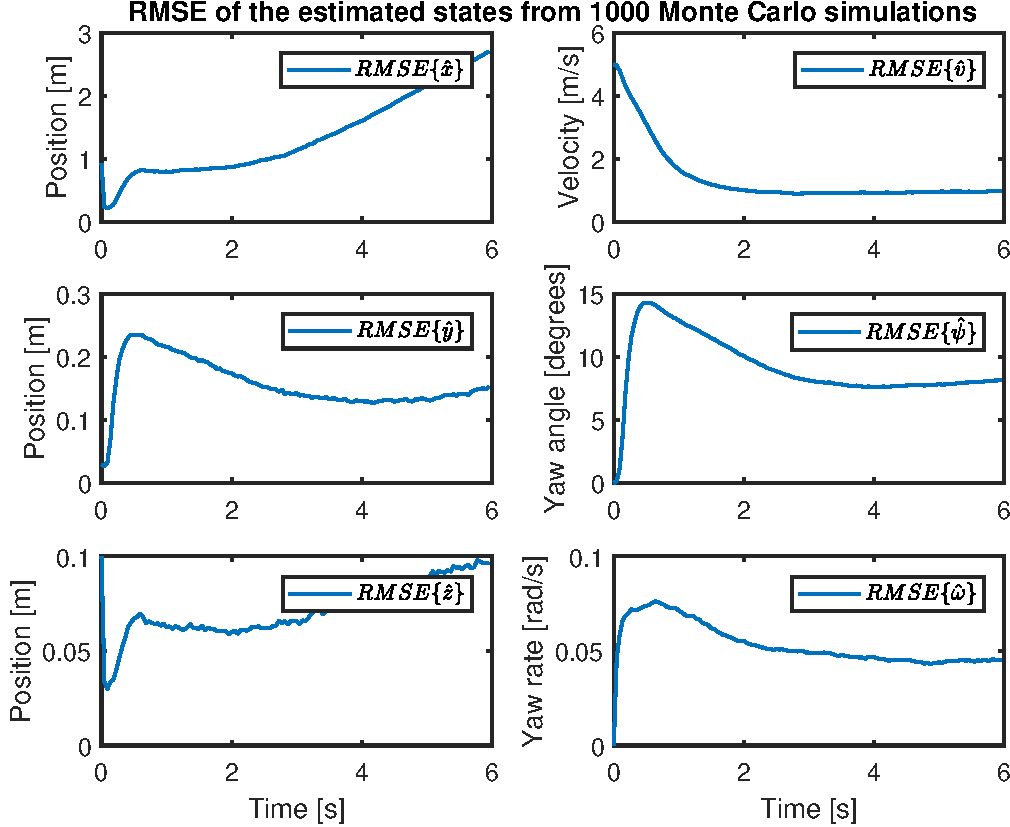
\includegraphics[width=0.8\textwidth]{MonteCarloSim/20_MC_1000_Rmse}
	\caption{\label{fig:20montesimstraighttowardsroiangvelrmse} Monte Carlo simulation result of scenario 1 with setup 2.}
\end{figure}

\begin{figure}[!ht]
	\centering
	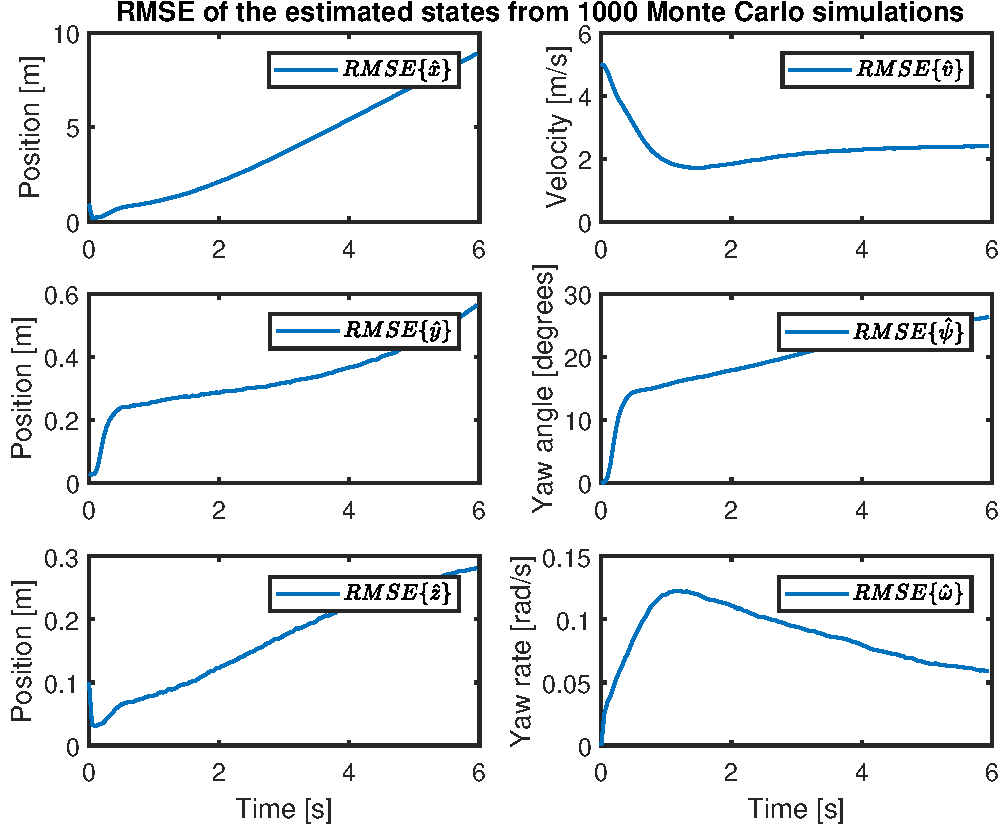
\includegraphics[width=0.8\textwidth]{MonteCarloSim/21_MC_1000_Rmse}
	\caption{\label{fig:21montesimstraighttowardsroiangvelrmse} Monte Carlo simulation result of scenario 1 with setup 3.}
\end{figure}

\begin{figure}[!ht]
	\centering
	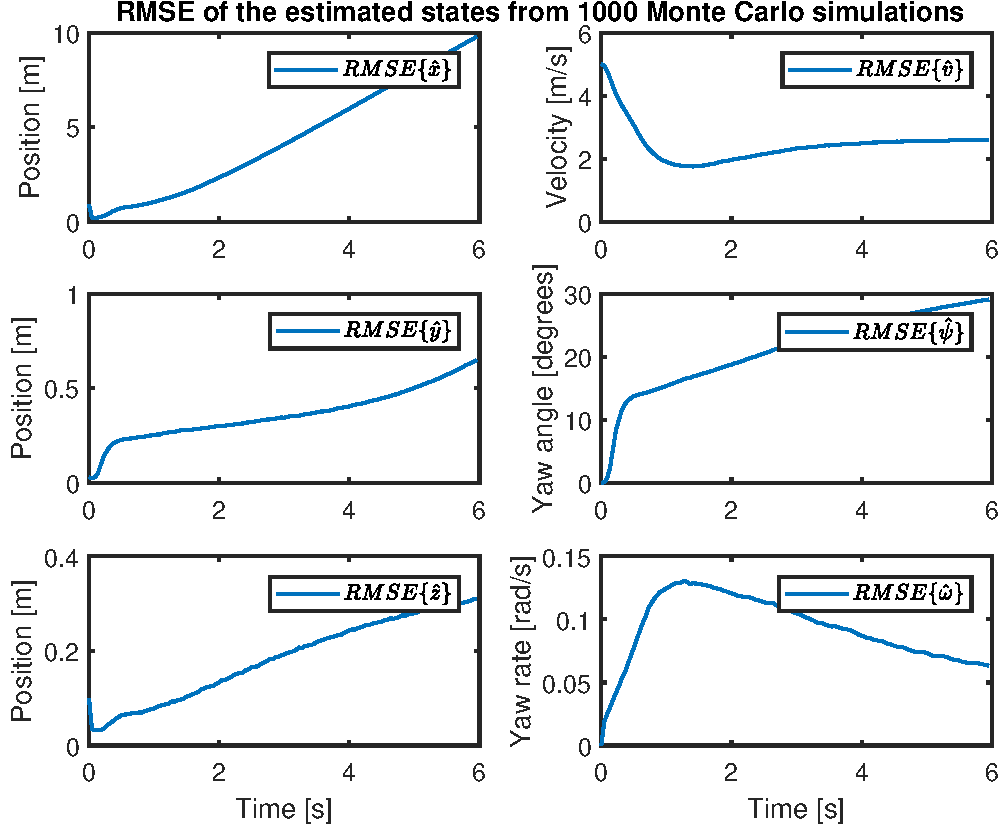
\includegraphics[width=0.8\textwidth]{MonteCarloSim/22_MC_1000_Rmse}
	\caption{\label{fig:22montesimstraighttowardsroiangvelrmse} Monte Carlo simulation result of scenario 1 with setup 4.}
\end{figure}

\begin{figure}[!ht]
	\centering
	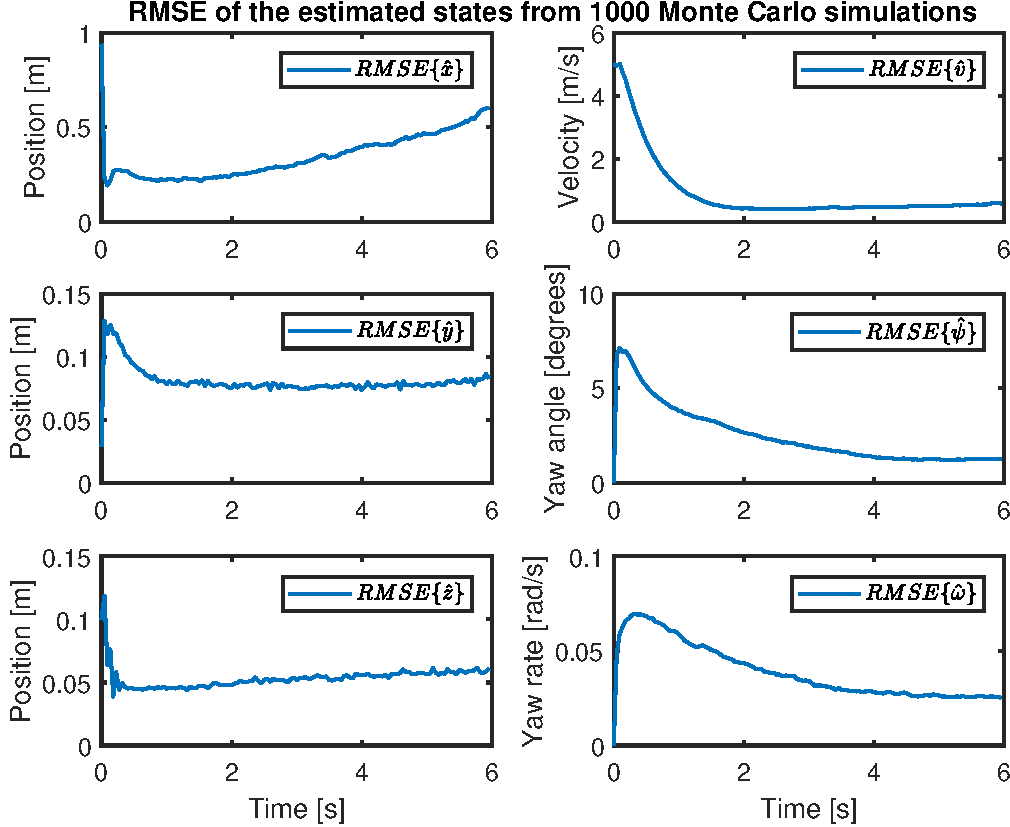
\includegraphics[width=0.8\textwidth]{MonteCarloSim/30_MC_1000_Rmse}
	\caption{\label{fig:30montesimstraighttowardsroiangvelcornerrmse} Monte Carlo simulation result of scenario 1 with setup 5.}
\end{figure}

\clearpage

Secondly, a simulation of a target (detected 15 meters in front of the host) performing a turn to the right, was evaluated.
The target drove with a constant velocity of 4 m/s and after 2 seconds, it performed a turn to the right.
The used measurements and the parameters $Q^\text{sim}_\omega$ and $R^\text{sim}_\omega$ varied according to \Tableref{tab:montesimscenario2}.

\begin{table}[!ht]
	\centering
	\caption{\label{tab:montesimscenario2} The simulation parameters and available measurements for different setup cases of the second simulated scenario.}
	\renewcommand{\arraystretch}{1.2}
	\begin{tabular}{|l|p{3.5cm}|l|l|}
		\hline
		\textbf{Setup no.} & \textbf{Measurements} & $Q^\text{sim}_\omega$ (rad/s) & $R^\text{sim}_\omega$ (rad/s) \\
		\hline
		6 & \abbrROI & $1.7\cdot 10^{-6}$ & -- \\
		\hline
		7 & \abbrROI and angular rate & $1.7\cdot 10^{-6}$ & 0.1 \\
		\hline
		8 & \abbrROI and angular rate & $1.7\cdot 10^{-6}$ & 0.5 \\
		\hline
		9 & \abbrROI and angular rate & $1.7\cdot 10^{-6}$ & 1 \\
		\hline
		10 & \abbrROI, angular rate and corners & $1.7\cdot 10^{-6}$ & 0.1 \\
		\hline
	\end{tabular}
\end{table}

In this scenario, the covariance matrices $\bm{Q}$ and $\bm{R}$ were
\begin{align}
	\label{eq:Qsim2}
	\bm{Q} &=
	\begin{pmatrix}
		0.25 & 0 & 0 & 0 & 0 & 0 \\
		0 & 0.1 & 0 & 0 & 0 & 0 \\
		0 & 0 & 0.05 & 0 & 0 & 0 \\
		0 & 0 & 0 & 1 & 0 & 0 \\
		0 & 0 & 0 & 0 & 0.00017 & 0 \\
		0 & 0 & 0 & 0 & 0 & 0.0017 \\
	\end{pmatrix}, \\
	\label{eq:Rsim2}
	\bm{R} &= 10 \bm{R}^\text{sim},
\end{align}
in all setup cases.
The matrix $\bm{R}^\text{sim}$ is given by \eqref{eq:Rsim}.

The results for each setup can be seen in \Figuresref{fig:13montesimcrossingroirmse}--\ref{fig:29montesimcrossingroiangvelcornerrmse}.
Examples of the simulated trajectories can be found in \Figuresref{fig:13trajectorycrossingroipos}--\ref{fig:29trajectorycrossingroiangvelcornerother} in \Appendixref{app:montecarlo}.

\Figureref{fig:13montesimcrossingroirmse} shows that if only \abbrROI measurements are used, a large \abbrRMSE were obtained of the estimated states.
The large \abbrRMSE of the angular rate state during the turn affects the rest of the states, especially the yaw angle.
In the simulation, as in the first scenario, the results are improved by adding angular rate measurements.
In \Figureref{fig:23montesimcrossingroiangvelrmse}, the angular rate noise variance level were 0.1 rad/s.
If the angular rate measurements had too high noise variance level, the \abbrRMSE of the estimated state started to diverge, as in \Figuresref{fig:24montesimcrossingroiangvelrmse} and \ref{fig:25montesimcrossingroiangvelrmse}.
The angular rate measurements variance noise levels were 0.5 rad/s and 1 rad/s, respectively.
As well as in the previous simulation, the result got significantly improved by adding the measurements of the target's corners, considering \Figureref{fig:29montesimcrossingroiangvelcornerrmse}.

\begin{figure}[!ht]
	\centering
	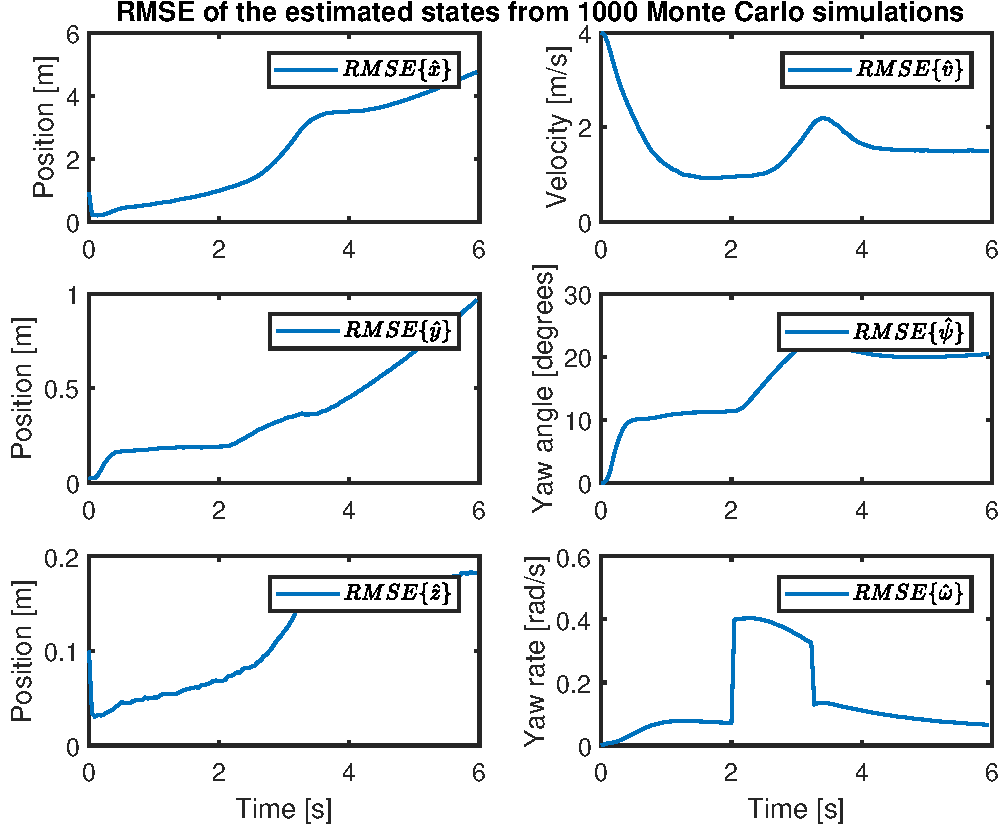
\includegraphics[width=0.8\textwidth]{MonteCarloSim/13_MC_1000_Rmse}
	\caption{\label{fig:13montesimcrossingroirmse} Monte Carlo simulation result of scenario 2 with setup 6.}
\end{figure}

\begin{figure}[!ht]
	\centering
	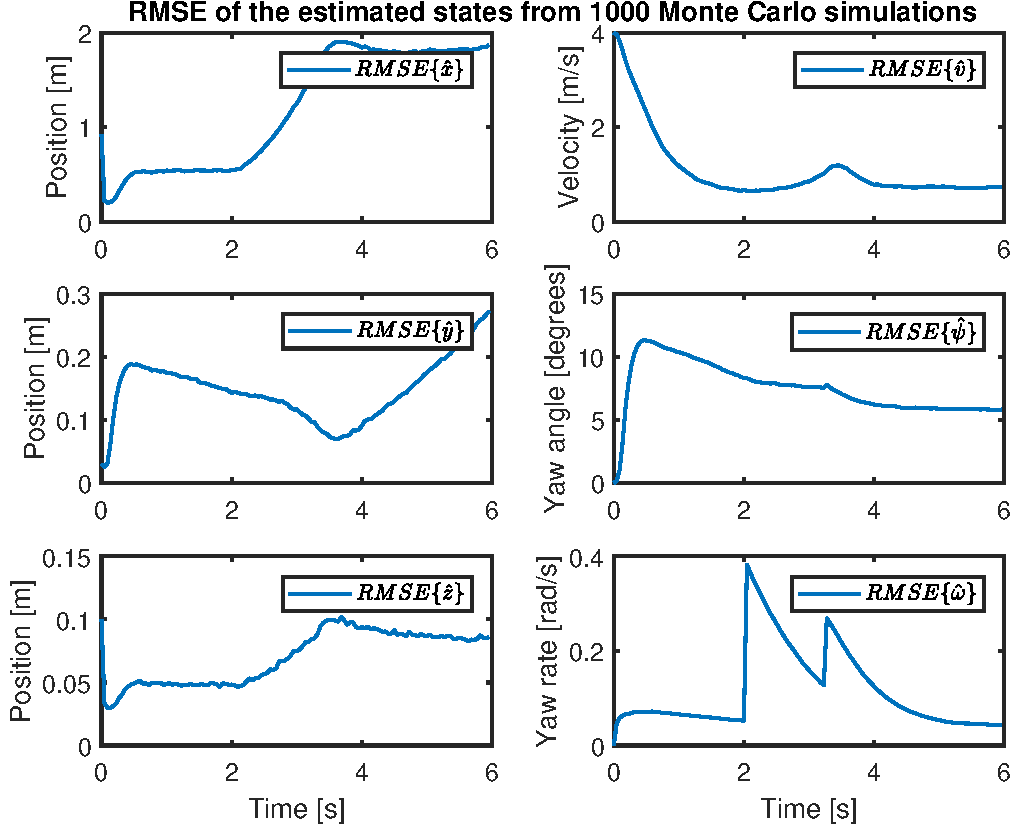
\includegraphics[width=0.8\textwidth]{MonteCarloSim/23_MC_1000_Rmse}
	\caption{\label{fig:23montesimcrossingroiangvelrmse} Monte Carlo simulation result of scenario 2 with setup 7.}
\end{figure}

\begin{figure}[!ht]
	\centering
	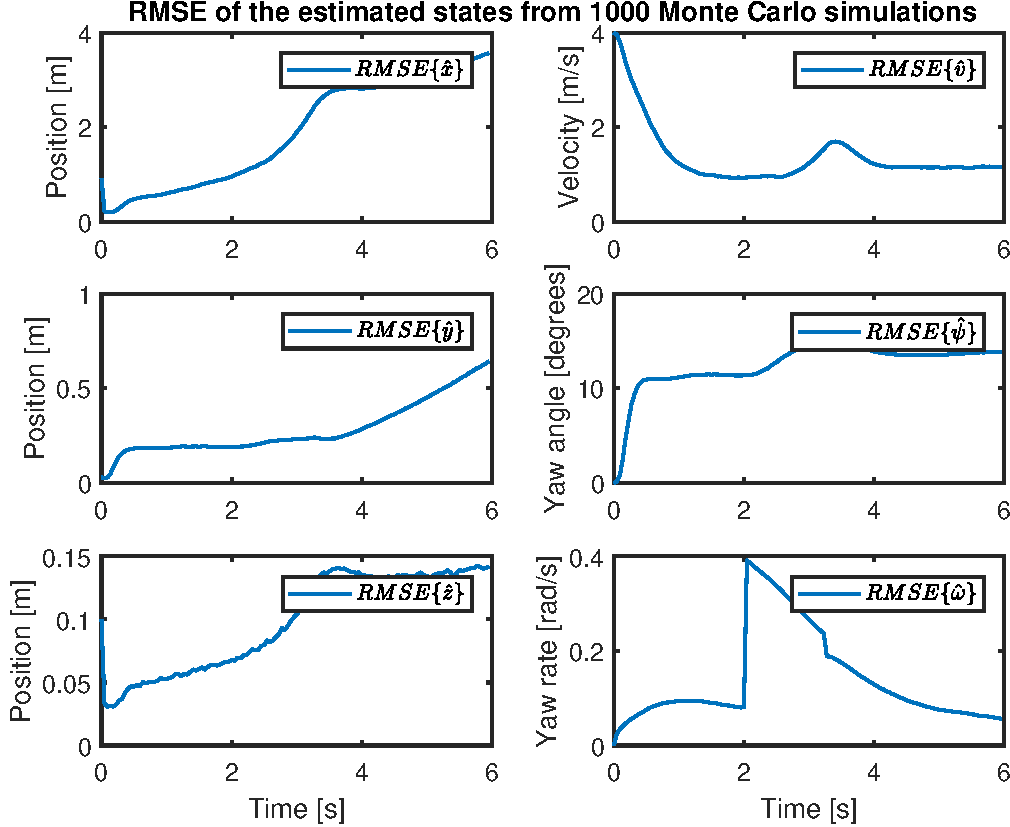
\includegraphics[width=0.8\textwidth]{MonteCarloSim/24_MC_1000_Rmse}
	\caption{\label{fig:24montesimcrossingroiangvelrmse} Monte Carlo simulation result of scenario 2 with setup 8.}
\end{figure}

\begin{figure}[!ht]
	\centering
	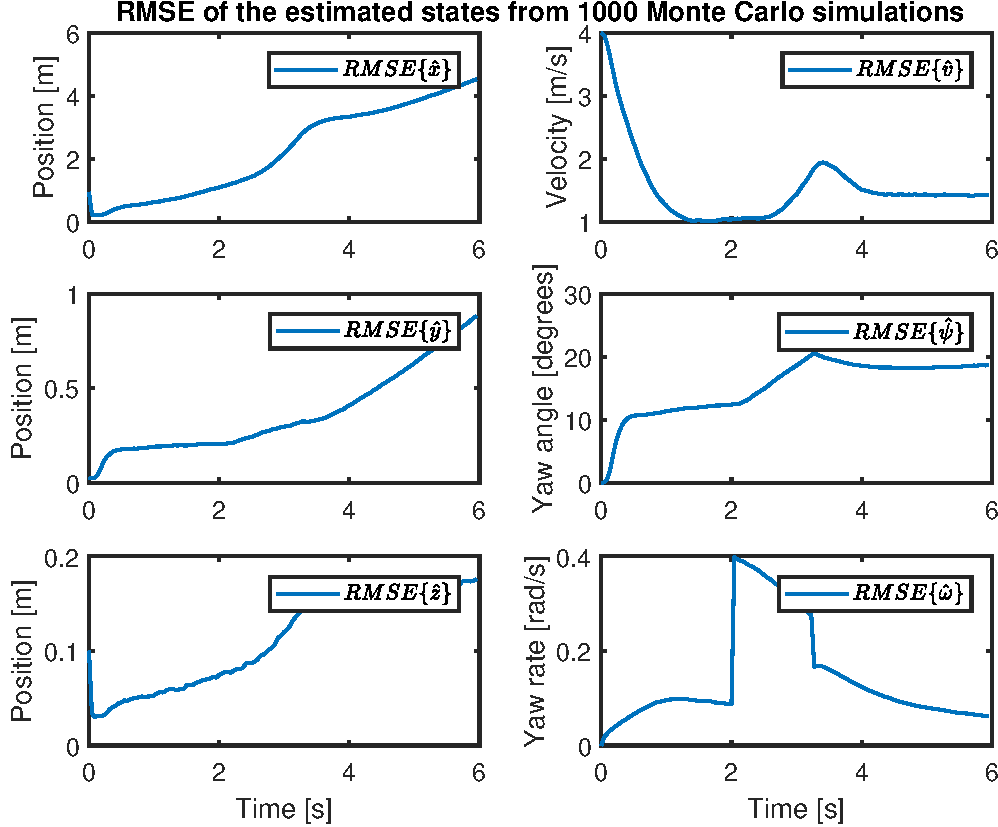
\includegraphics[width=0.8\textwidth]{MonteCarloSim/25_MC_1000_Rmse}
	\caption{\label{fig:25montesimcrossingroiangvelrmse} Monte Carlo simulation result of scenario 2 with setup 9.}
\end{figure}

\begin{figure}[!ht]
	\centering
	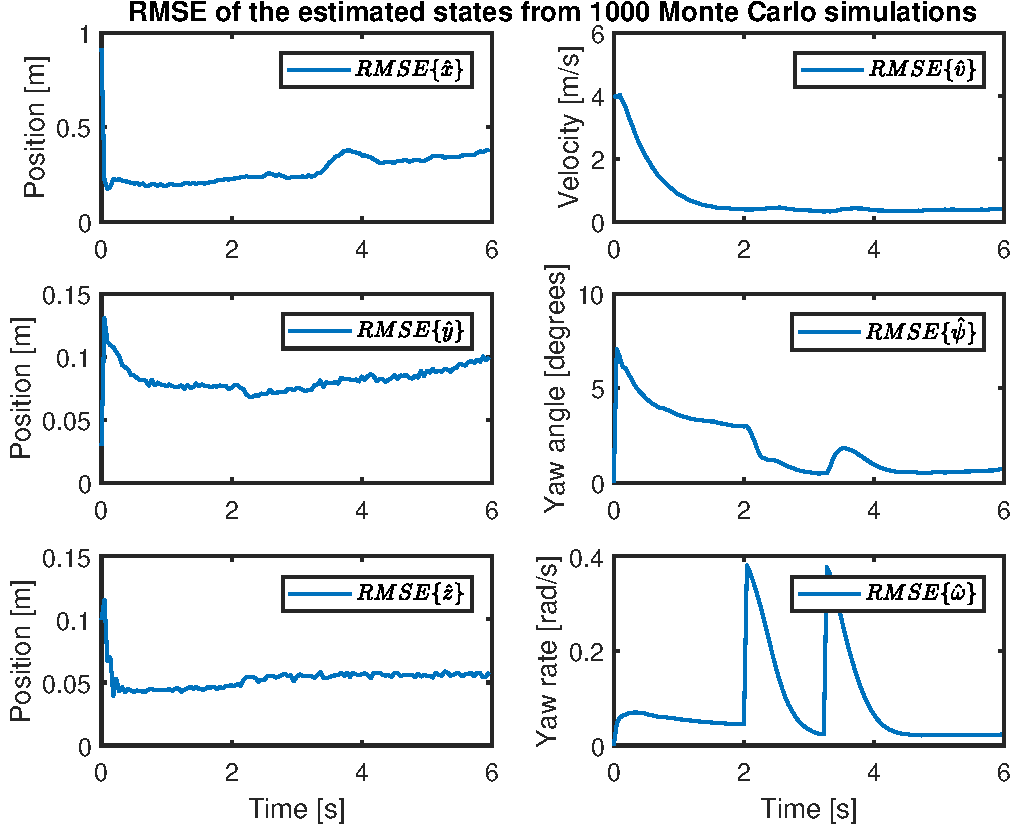
\includegraphics[width=0.8\textwidth]{MonteCarloSim/29_MC_1000_Rmse}
	\caption{\label{fig:29montesimcrossingroiangvelcornerrmse} Monte Carlo simulation result of scenario 2 with setup 10.}
\end{figure}

\newpage

The purpose of performing Monte Carlo simulations were to show which performance, \ie measurement noise level, that must be achieved in order to produce a good state estimated with the proposed filter structure.
This was especially interesting for the angular rate measurements.
From the two simulated scenarios, the results have shown that a measurement variance of 0.1 rad/s for the angular rate should be good enough.
A measurement noise variance of 0.5 rad/s is too large in order to obtain a good state estimate.

\newpage

\section{Homography Estimation}
\label{sec:homographyestimationresults}
It is of great interest to see how good homography estimates that can be achieved.
As can be seen from the Monte Carlo simulations in \Sectionref{sec:montecarloresult}, the angular rate measurements have the possibility to improve the result, if they have a low enough noise level.

Some experimentation on synthetic data has been performed in order to evaluate the result of the homography estimations.
A rectangle was created, and it used the same motion model as described in \eqref{eq:motionmodel}, to represent the possible backside of a target vehicle.
The tracked points on the rectangle were the four corner points and an additional number of randomly selected uniformly distributed points on the rectangle.
The rectangle performed a trajectory where it travelled straight away and then turned left.
In order to perturb the synthetic data, Gaussian noise was added when projecting the points on the rectangle onto the image plane.
This will make the points not to lie perfectly on the same plane.

To perform the homography estimation, \matlab mex functions that interfaced the OpenCV library \cite{mexopencv} were used, both when estimating the homography matrix $\bm{H}$ and when performing the decomposition into $\rotmat, \bm{t}$ and $\bm{n}$.

The results of the synthetic data simulation can be seen in \Figuresref{fig:rectsim1e-2}--\ref{fig:rectsim5e-1}.
Different noise levels were used in each of the four simulations.
In the four simulations, 30 points were tracked inside the rectangle.
The rectangle was travelling with a constant velocity of 5 m/s and between frame number 35 and 65 it performed a turn with a constant angular rate of 0.25 rad/s.
The distance travelled was between 5 to 30 meters.

By observing the result from the homography estimation with synthetic data, several things can be stated:
\begin{itemize}
	\item If the matching pixels do not match well enough, \ie the errors in matched pixel coordinates are too large, the quality of the estimated homography will be reduced.
	\item At a distance further away, the mismatching pixels will have an even larger effect on the homography estimation.
	\item If the target is far away, not even a small mismatch error might be good enough for estimating the homography, since the true movement of the feature points is small.
\end{itemize}

The same method was used when constructing the angular rate measurements from real-world data.
\Figureref{fig:angvelmeas} shows the angular rate measurements constructed from the estimated homographies with real-world data.
In \Figureref{fig:angvelmeas155532}, one can see that the angular rate measurements have a trend around 0 rad/s.
\Figureref{fig:angvelmeas155733} shows a negative trend of the angular rate measurements, since the target vehicle is turning to the right.
In order to have a comparison, the estimated angular rate state from a stereo camera system is shown in the same figure.

Looking at \Figureref{fig:angvelmeas}, some reasonable explanations to the noisy results could be that the feature point tracker does not perform well enough or that the selected feature point detector did not detect enough feature points.
Another explanation might be that the OpenCV implementation for finding and decomposing the homography matrix is too sensitive to noise, even though a \abbrRANSAC method (see \Sectionref{sec:ransac}) was utilized.

By further analysing the angular rate measurements from \Figureref{fig:angvelmeas}, their respectively variances could be calculated.
For the first sequence, a linear trend was subtracted from the measurements and the resulting variance was 0.8 rad/s.
For the seconds sequence, a nonlinear trend was subtracted from the measurements and the resulting variance was 2 rad/s.
These variances are too high compared to the required variance discussed in the previous section.
The evaluated sequences were recorded in clear daylight.
It is reasonable to believe that the feature points will be even more difficult to track in bad light or in bad weather conditions.

The detection and tracking of feature points were implemented using \matlab's computer vision system toolbox.
For feature point detection, the minimum eigenvalue algorithm \cite{mineigendetector:2018} and the Harris–Stephens algorithm \cite{harrisdetector:2018} were used.
For feature point tracking, the KLT feature point tracker \cite{pointtracker:2018} was used.

A potential error source is the spatial location of the detected feature points.
In \cite{Bostanci:2012}, it is emphasized that the spatial location of the feature points affects the accuracy of the homography estimation.
By selecting different feature point detectors, a different result might have been obtained.
Dividing the \abbrROI into smaller sized rectangles and by running different detectors until a suitable number of feature points have been detected might be one way of ensuring better spatial location.

From the synthetic data experiment, it turned out that the best approach to the homography decomposition (see \Sectionref{sec:angratemeas}) was to choose the largest of the two final solutions.
This method was then utilized when running the algorithm on real-world data.
It might be that this method is not the correct way of selecting the final solution, when also dealing with bad feature point correspondence.

\clearpage

\begin{figure}[!ht]
	\centering
	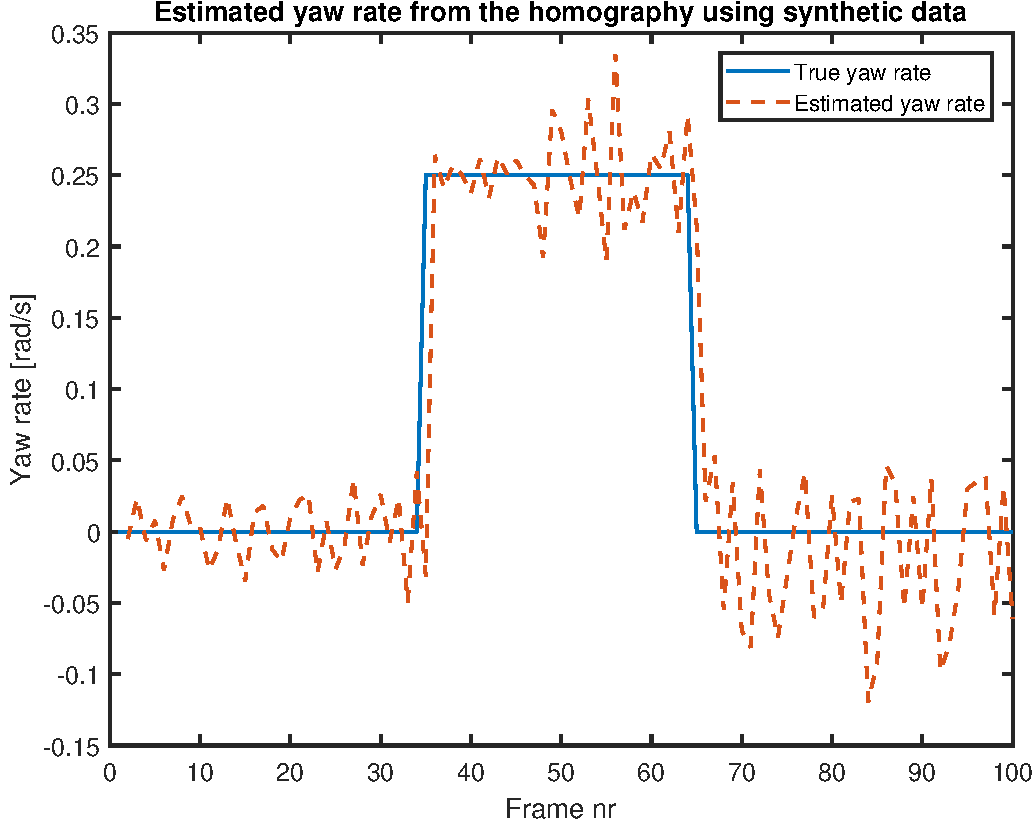
\includegraphics[width=0.7\textwidth]{RectangleSim/rect_1e-2}
	\caption{\label{fig:rectsim1e-2} Simulation result with synthetic data from a travelling rectangle. Here, Gaussian noise with a standard deviation of 0.01 pixels was added when the points on the rectangle were projected into the image plane.}
\end{figure}

\begin{figure}[!ht]
	\centering
	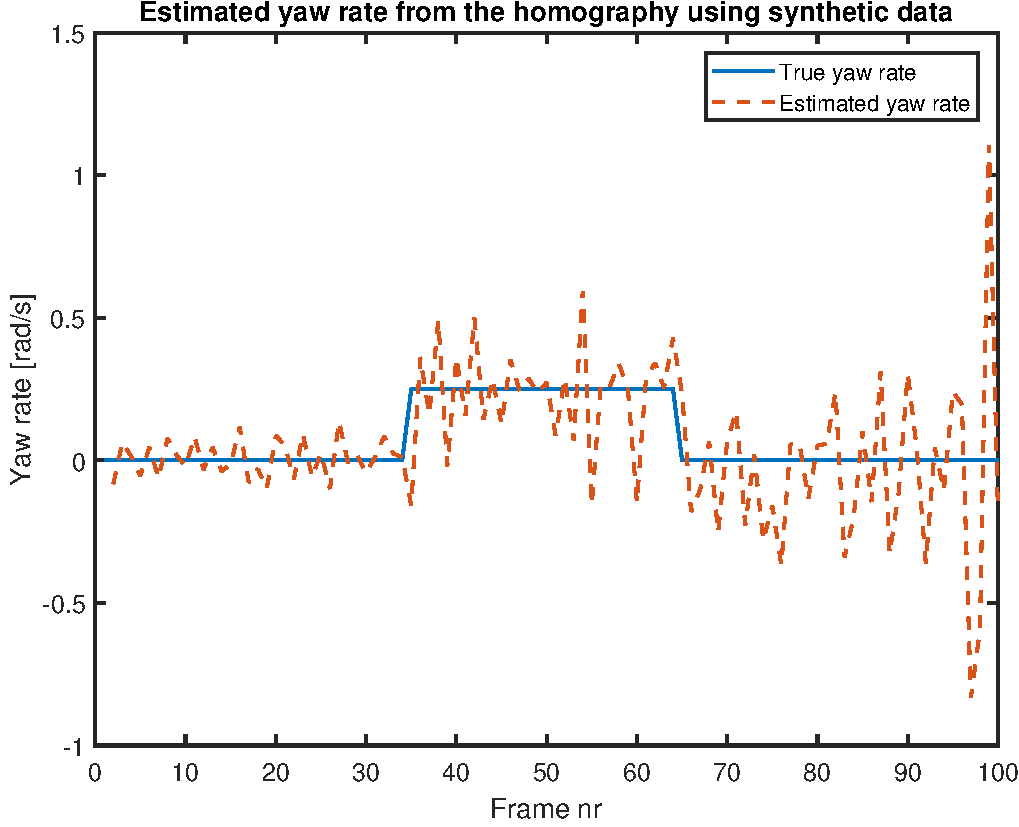
\includegraphics[width=0.7\textwidth]{RectangleSim/rect_5e-2}
	\caption{\label{fig:rectsim5e-2} Simulation result with synthetic data from a travelling rectangle. Here, Gaussian noise with a standard deviation of 0.05 pixels was added when the points on the rectangle were projected into the image plane.}
\end{figure}

\begin{figure}[!ht]
	\centering
	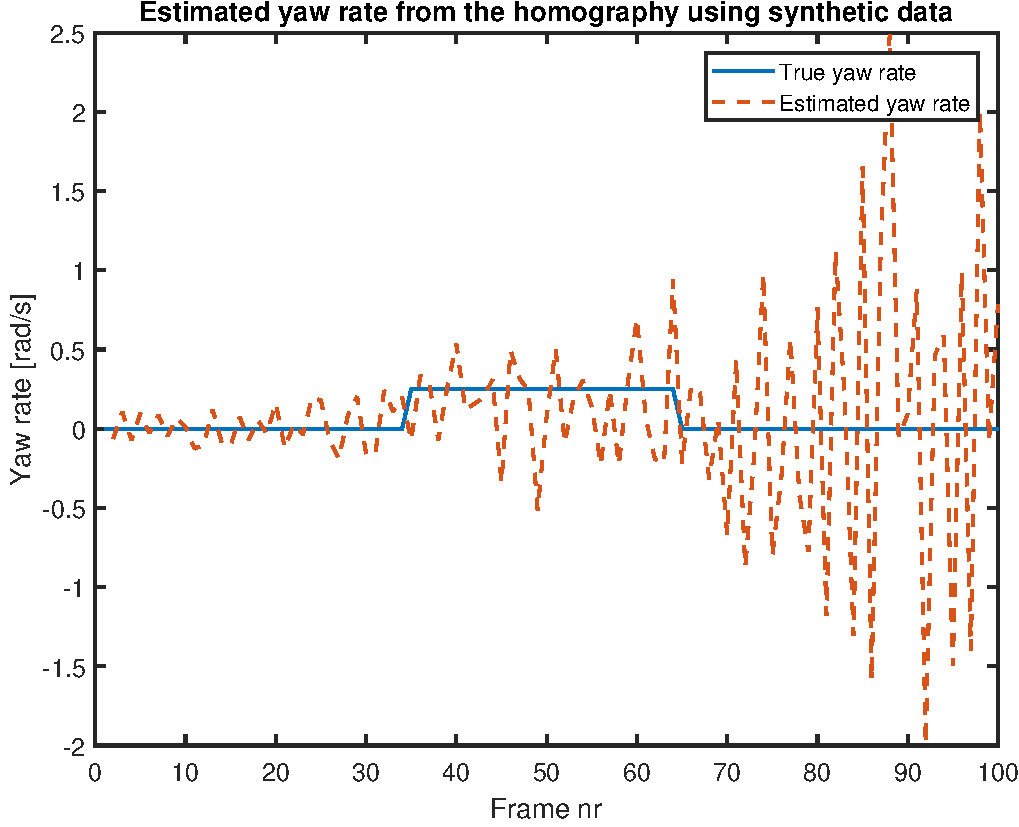
\includegraphics[width=0.7\textwidth]{RectangleSim/rect_1e-1}
	\caption{\label{fig:rectsim1e-1} Simulation result with synthetic data from a travelling rectangle. Here, Gaussian noise with a standard deviation of 0.1 pixels was added when the points on the rectangle were projected into the image plane.}
\end{figure}

\begin{figure}[!ht]
	\centering
	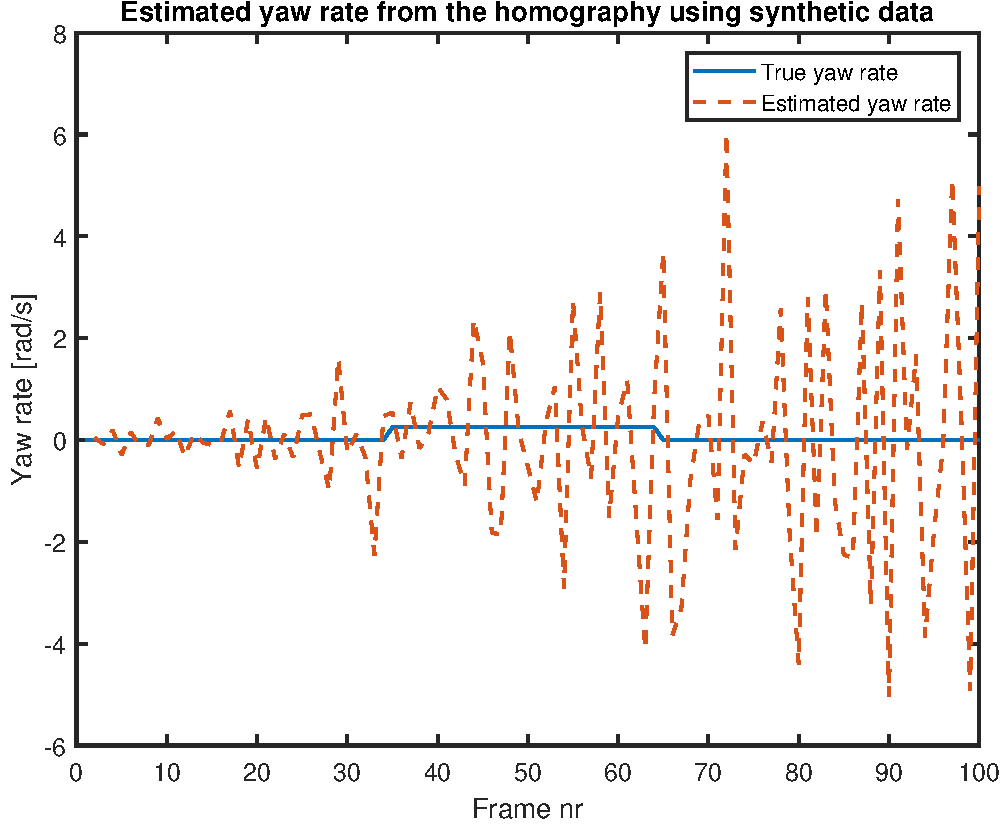
\includegraphics[width=0.7\textwidth]{RectangleSim/rect_5e-1}
	\caption{\label{fig:rectsim5e-1} Simulation result with synthetic data from a travelling rectangle. Here, Gaussian noise with a standard deviation of 0.5 pixels was added when the points on the rectangle were projected into the image plane.}
\end{figure}

\begin{figure}[!ht]
	\centering
	\subfloat[][Constructed angular rate measurements for the first sequence.]
	{
		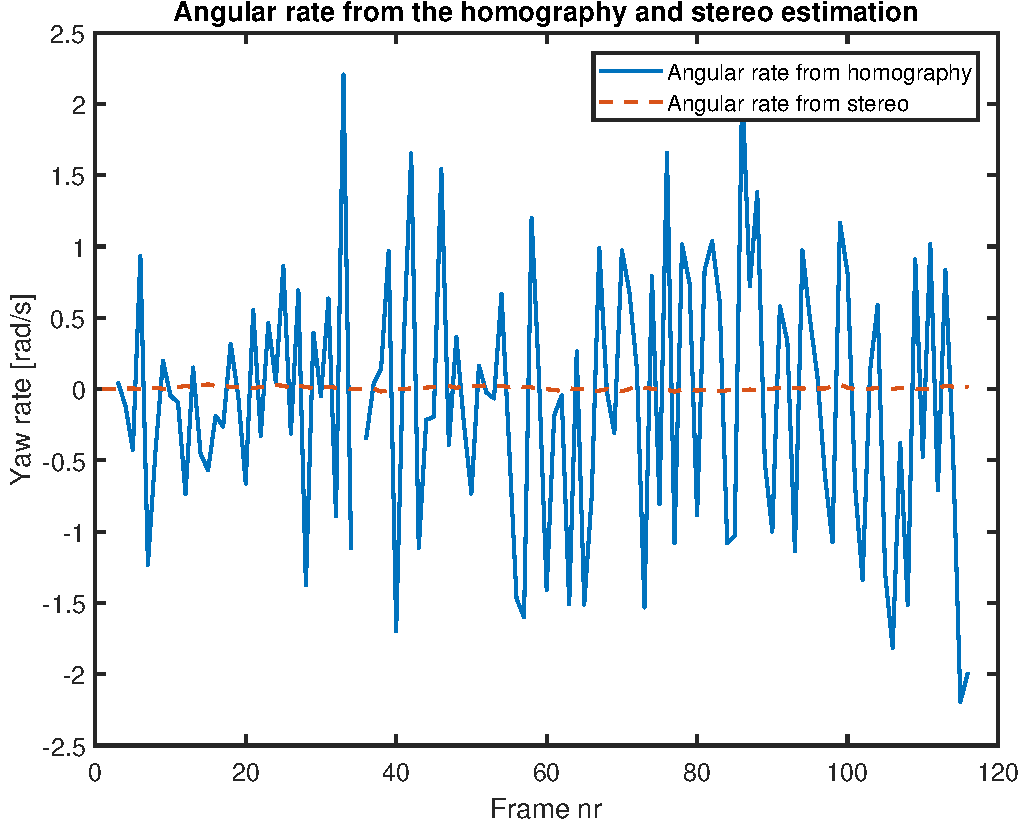
\includegraphics[width=0.7\textwidth]{StereoComparison/155532_AngVelComparison}
		\label{fig:angvelmeas155532}
	}

	\subfloat[][Constructed angular rate measurements for the second sequence.]
	{
		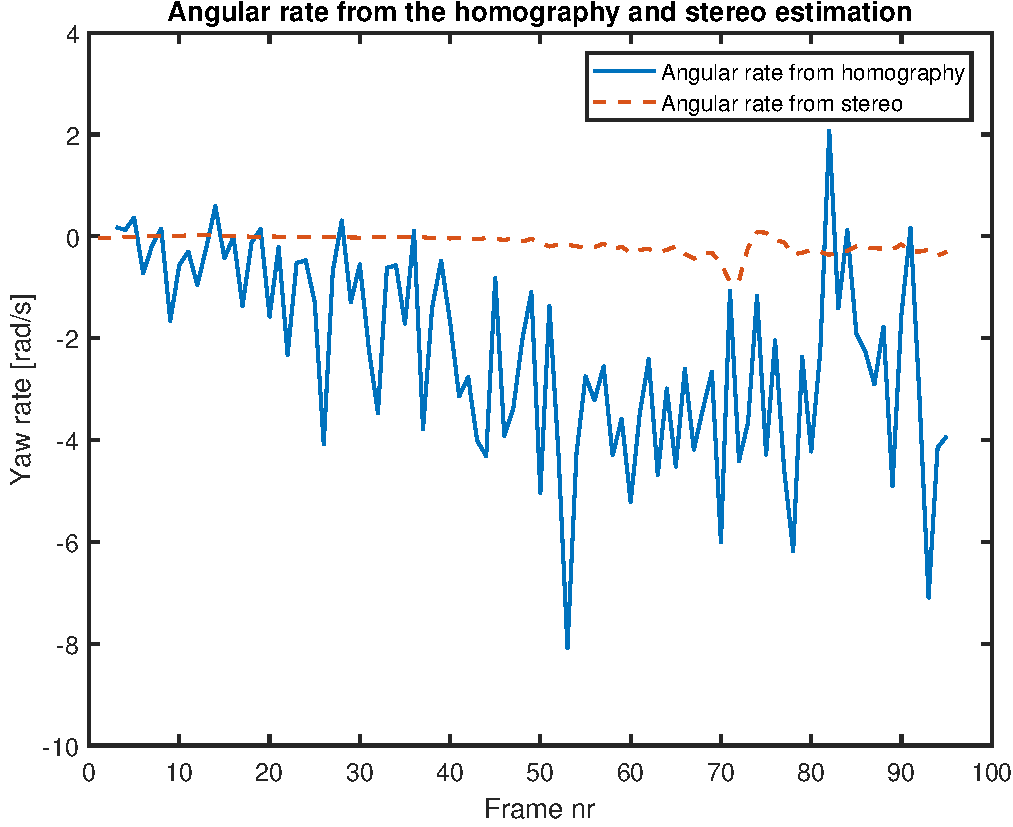
\includegraphics[width=0.7\textwidth]{StereoComparison/155733_AngVelComparison}
		\label{fig:angvelmeas155733}
	}
	\caption{\label{fig:angvelmeas} Angular rate measurements constructed from homography estimations. As a comparison, the estimated angular rate from a stereo camera system is shown as well.}
\end{figure}

\clearpage

\section{Comparison with a Stereo Camera System}
One of the goals with this \ms was to evaluate the performance of the mono tracker constructed in this thesis with a stereo system.
For this purpose, real-world data were collected with a stereo camera system to use as ground truth.
The two sequences, which a comparison has been performed with, are shown in \Figuresref{fig:sequence155532} and \ref{fig:sequence155733}.
The first sequence contains a target which travels straight forward and the second sequence contains a target which makes a turn to the right.

The resulting state comparisons are presented in \Figuresref{fig:comparison155532} and \ref{fig:comparison155733}.
The estimated states from the stereo camera had poor performance in some parts of the sequence.
In the first sequence, the poor stereo state estimates in $x$ and $\psi$ around frame number 100 gave a large error in the comparison.
In the second sequence, the poor stereo states estimates in $v$ and $\omega$ around frame number 72 gave a large error in the comparison.

When the target is travelling straight, there is less performance to gain by adding the corners as measurements compared to just using the \abbrROI and angular rate as measurements.
Compare \Figureref{fig:roiangvel155532} with \Figuresref{fig:roicorner155532} and \ref{fig:all155532}.
This might depend on that the generated angular rate measurements were better for this particular scenario, see \Figureref{fig:angvelmeas155532}, than for the turning scenario in \Figureref{fig:angvelmeas155733}.

By looking in \Figureref{fig:angvelmeas155733}, one can see that the angular rate measurements overestimates the turning rate.
Therefore, the filter was tuned with a high variance for the angular rate measurement in the measurement noise covariance matrix $\bm{R}$.
In this sequence, the state estimate gets improved by substituting the angular rate for corner measurements.
Compare \Figureref{fig:roiangvel155733} with \Figureref{fig:roicorner155733} and especially note the improvement of the yaw angle towards the end of the sequence.
From frame number 60, three corners of the target were visible which improved the orientation estimation.
When all three measurements are combined, in \Figureref{fig:all155733}, a similar result to \Figureref{fig:roicorner155733} is obtained.

\begin{figure}[!ht]
	\centering
	\subfloat[][Frame number 1.]
	{
		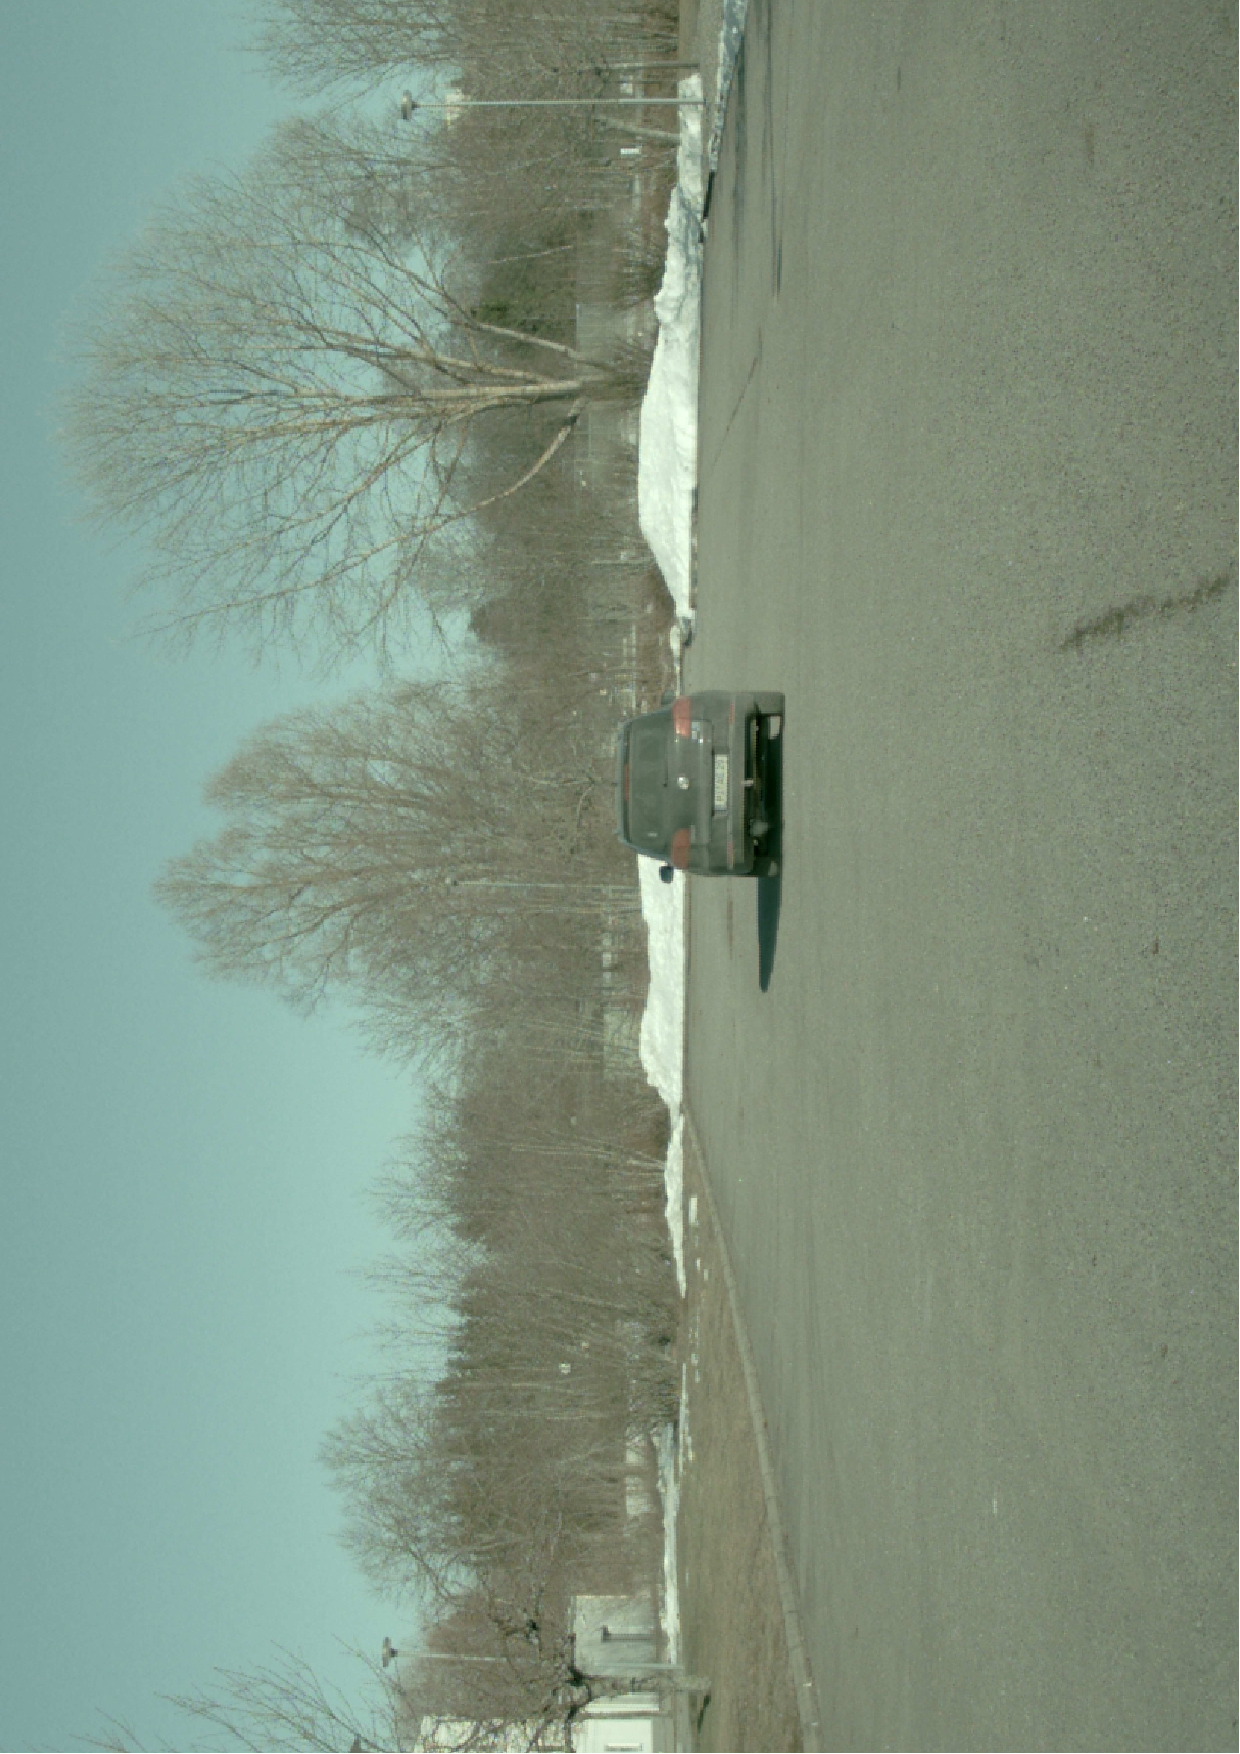
\includegraphics[angle=-90,origin=c,trim={0 0 5cm 0},width=0.55\textwidth]{Sequences/155532_1}
		\label{fig:155532_1}
	}

	\subfloat[][Frame number 45.]
	{
		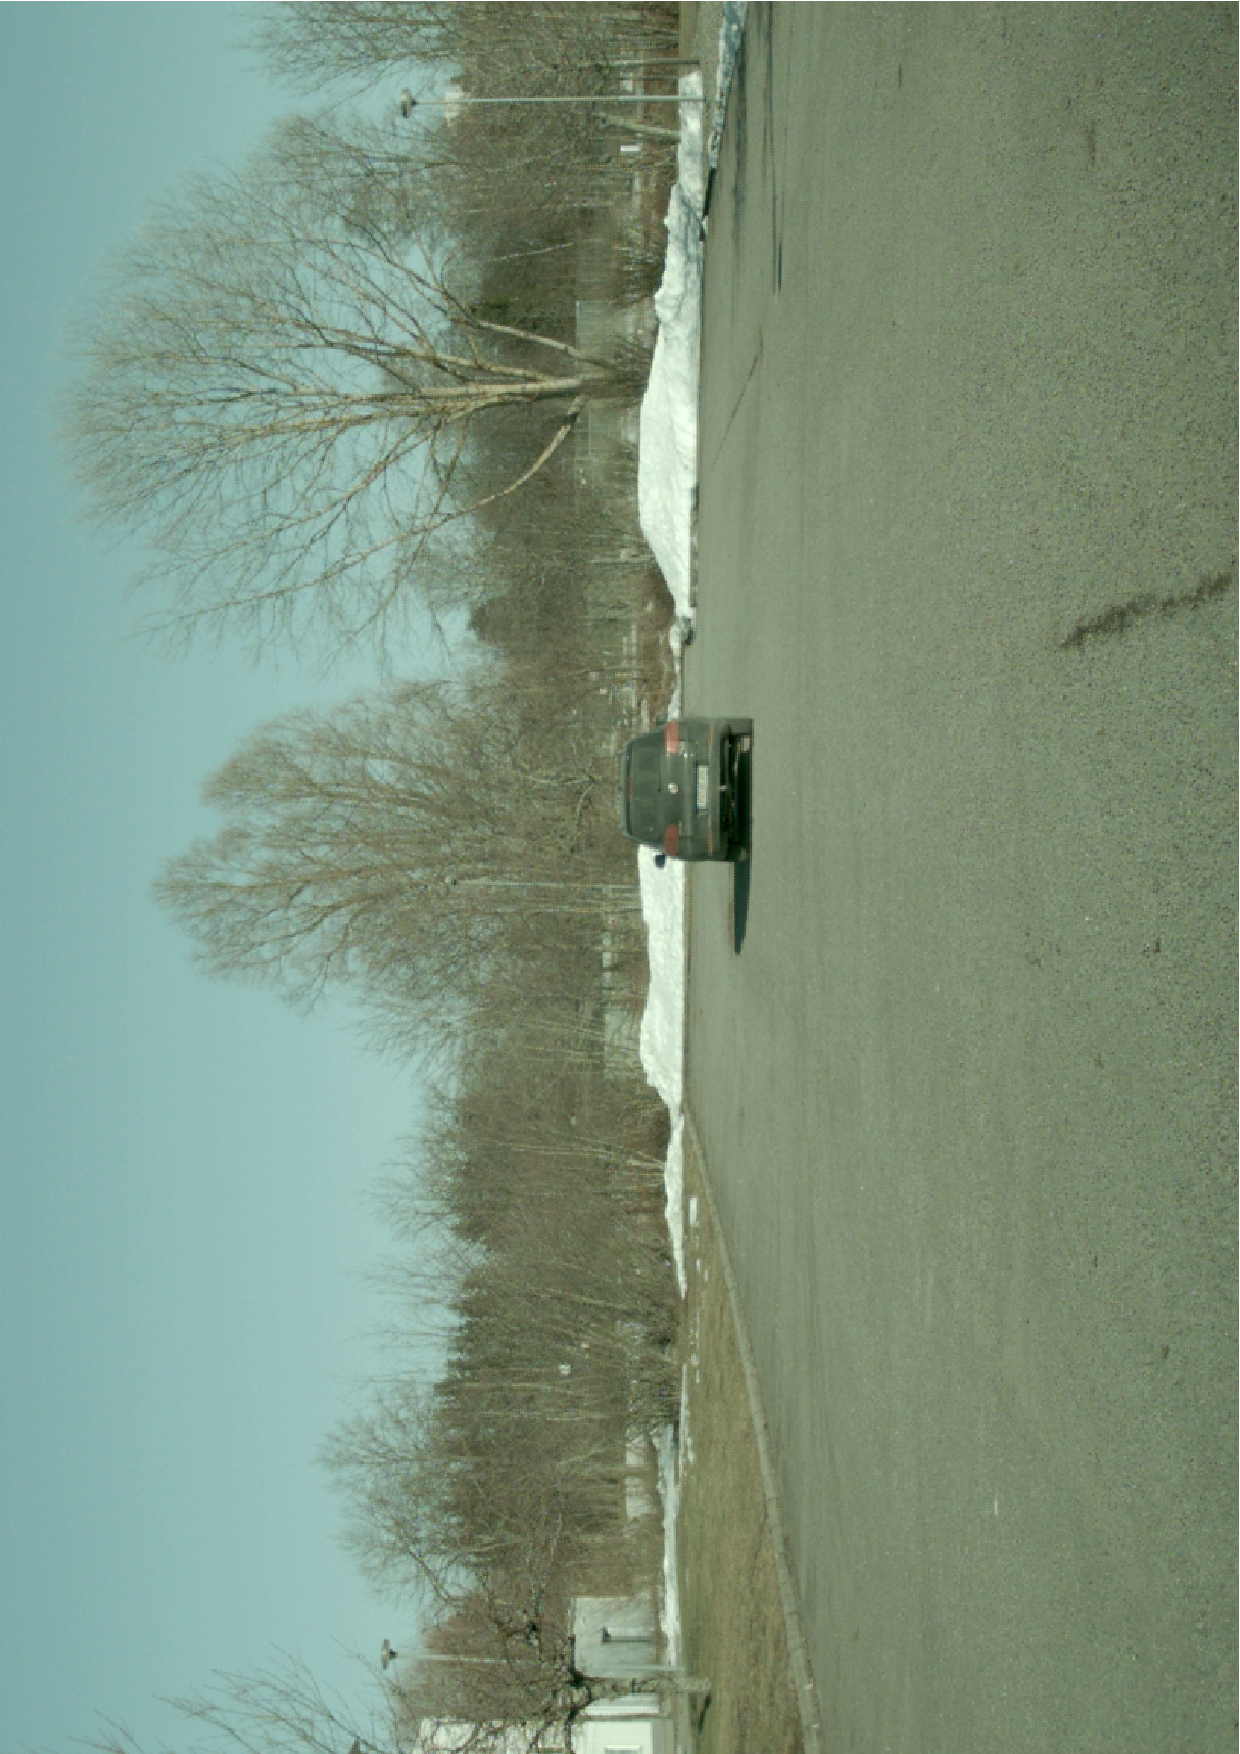
\includegraphics[angle=-90,origin=c,trim={0 0 5cm 0},width=0.55\textwidth]{Sequences/155532_45}
		\label{fig:155532_45}
	}

	\subfloat[][Frame number 95.]
	{
		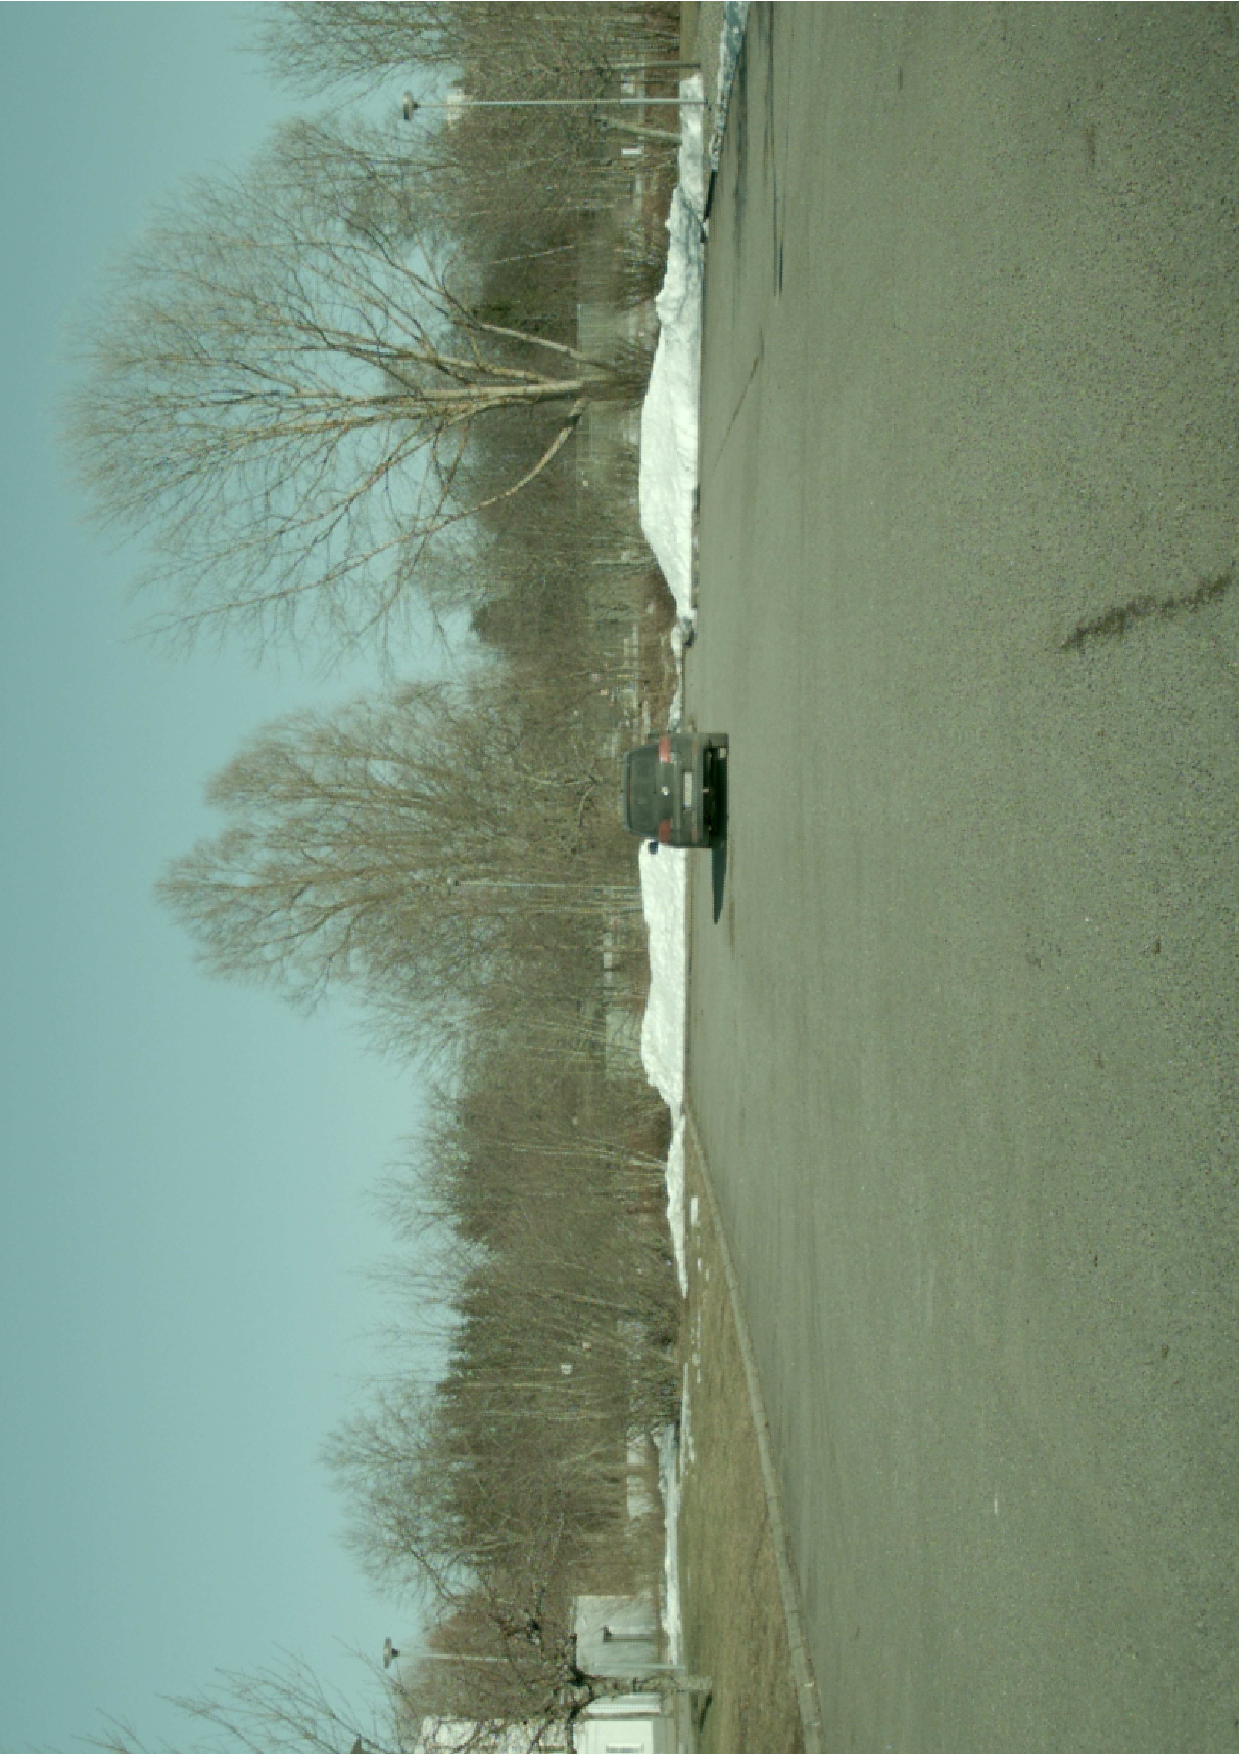
\includegraphics[angle=-90,origin=c,trim={0 0 5cm 0},width=0.55\textwidth]{Sequences/155532_95}
		\label{fig:155532_95}
	}
	\caption{\label{fig:sequence155532} The first sequence where the target vehicle drives straight forward, away from the host.}
\end{figure}

\begin{figure}[!ht]
	\centering
	\subfloat[][Frame number 20.]
	{
		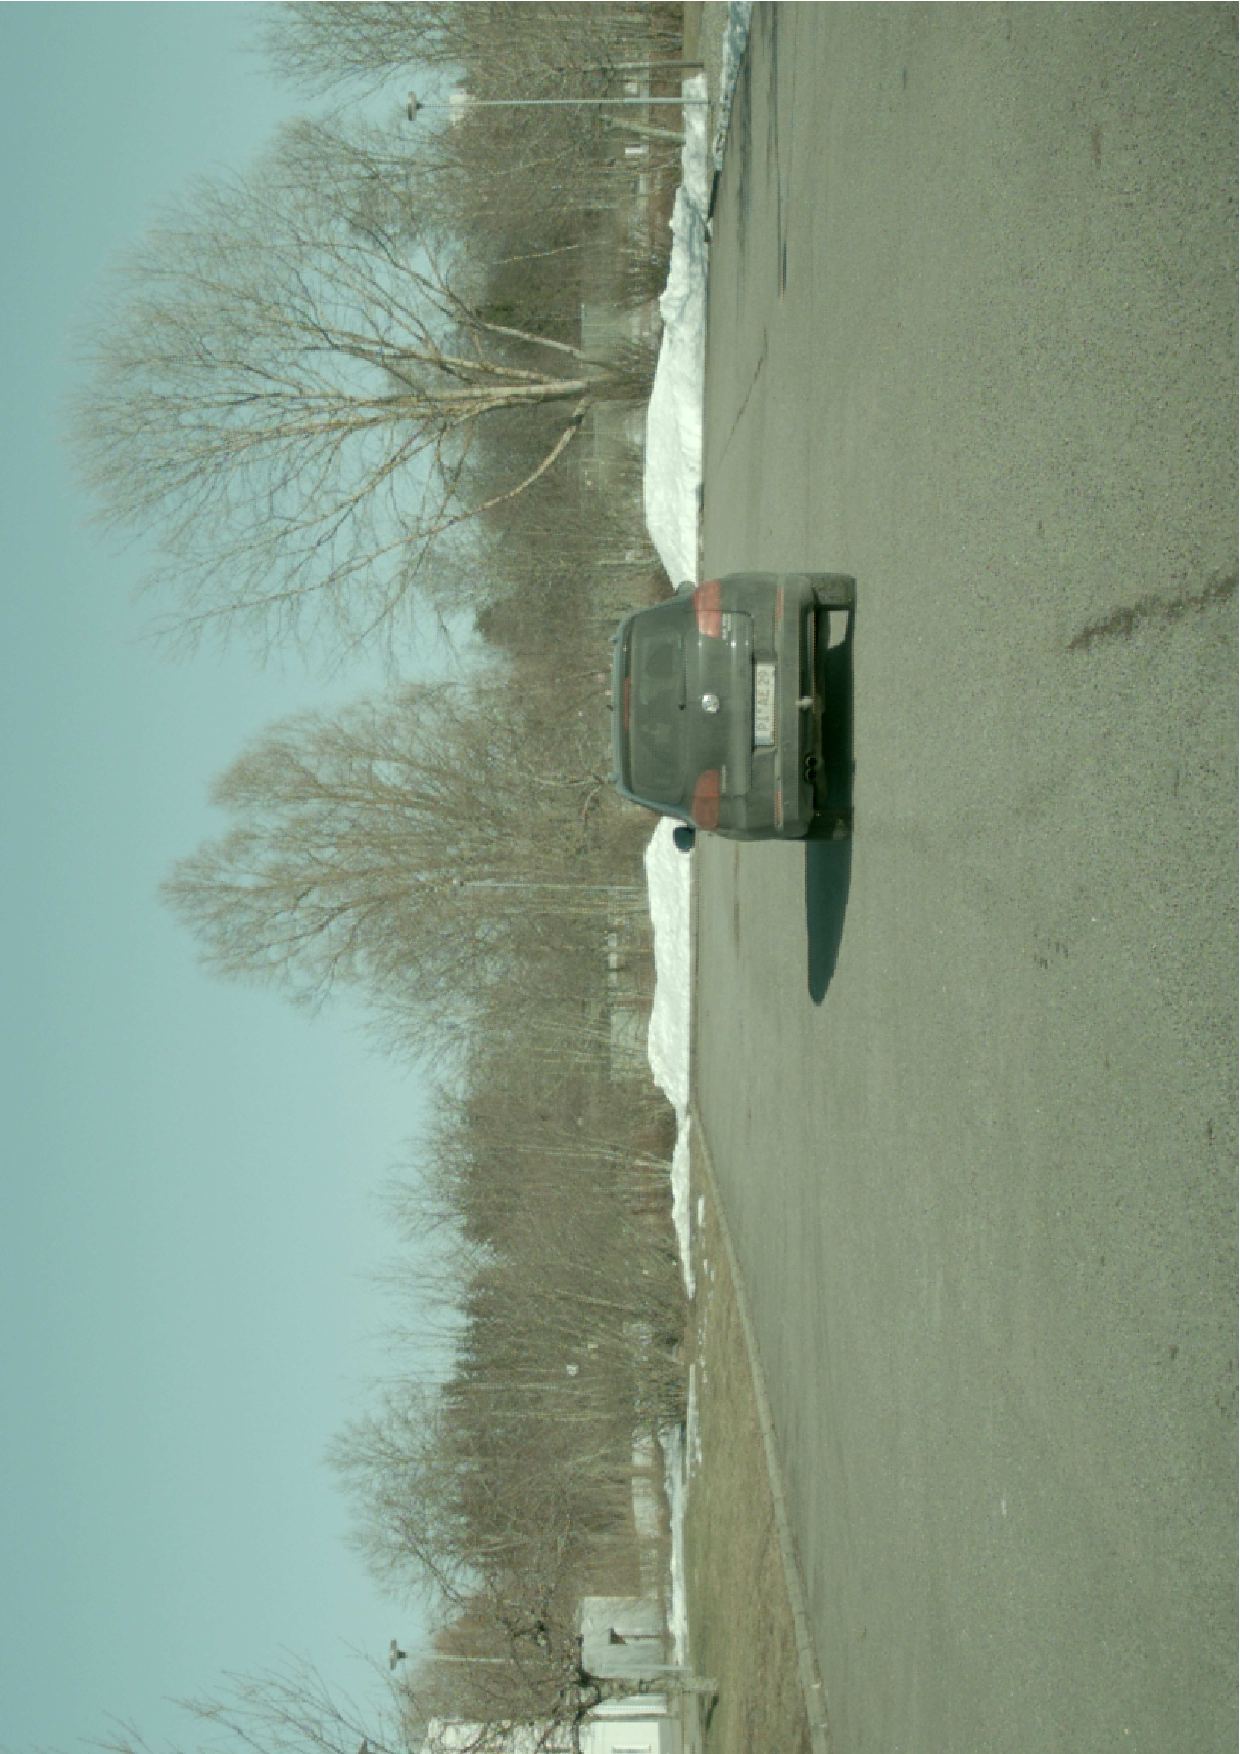
\includegraphics[angle=-90,origin=c,trim={0 0 5cm 0},width=0.55\textwidth]{Sequences/155733_20}
		\label{fig:155733_20}
	}

	\subfloat[][Frame number 55.]
	{
		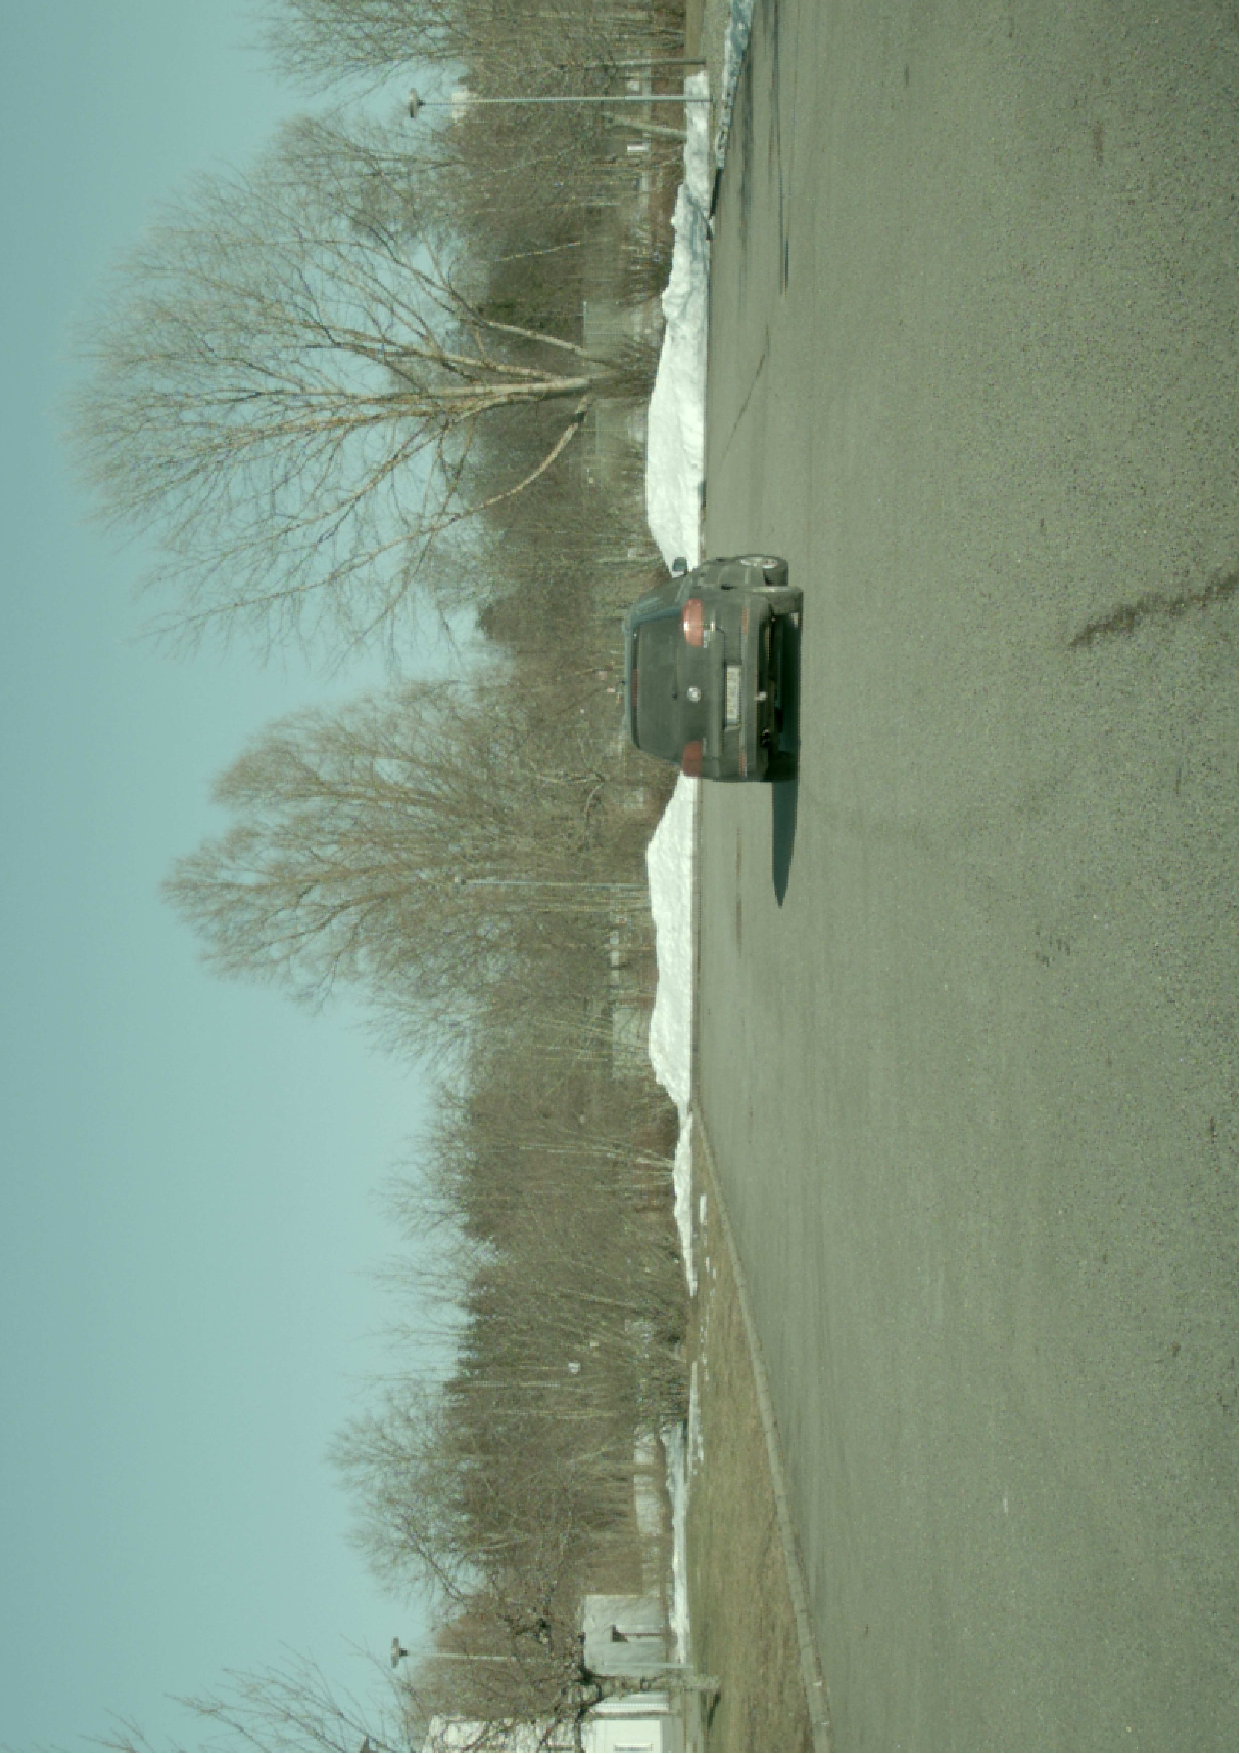
\includegraphics[angle=-90,origin=c,trim={0 0 5cm 0},width=0.55\textwidth]{Sequences/155733_55}
		\label{fig:155733_55}
	}

	\subfloat[][Frame number 95.]
	{
		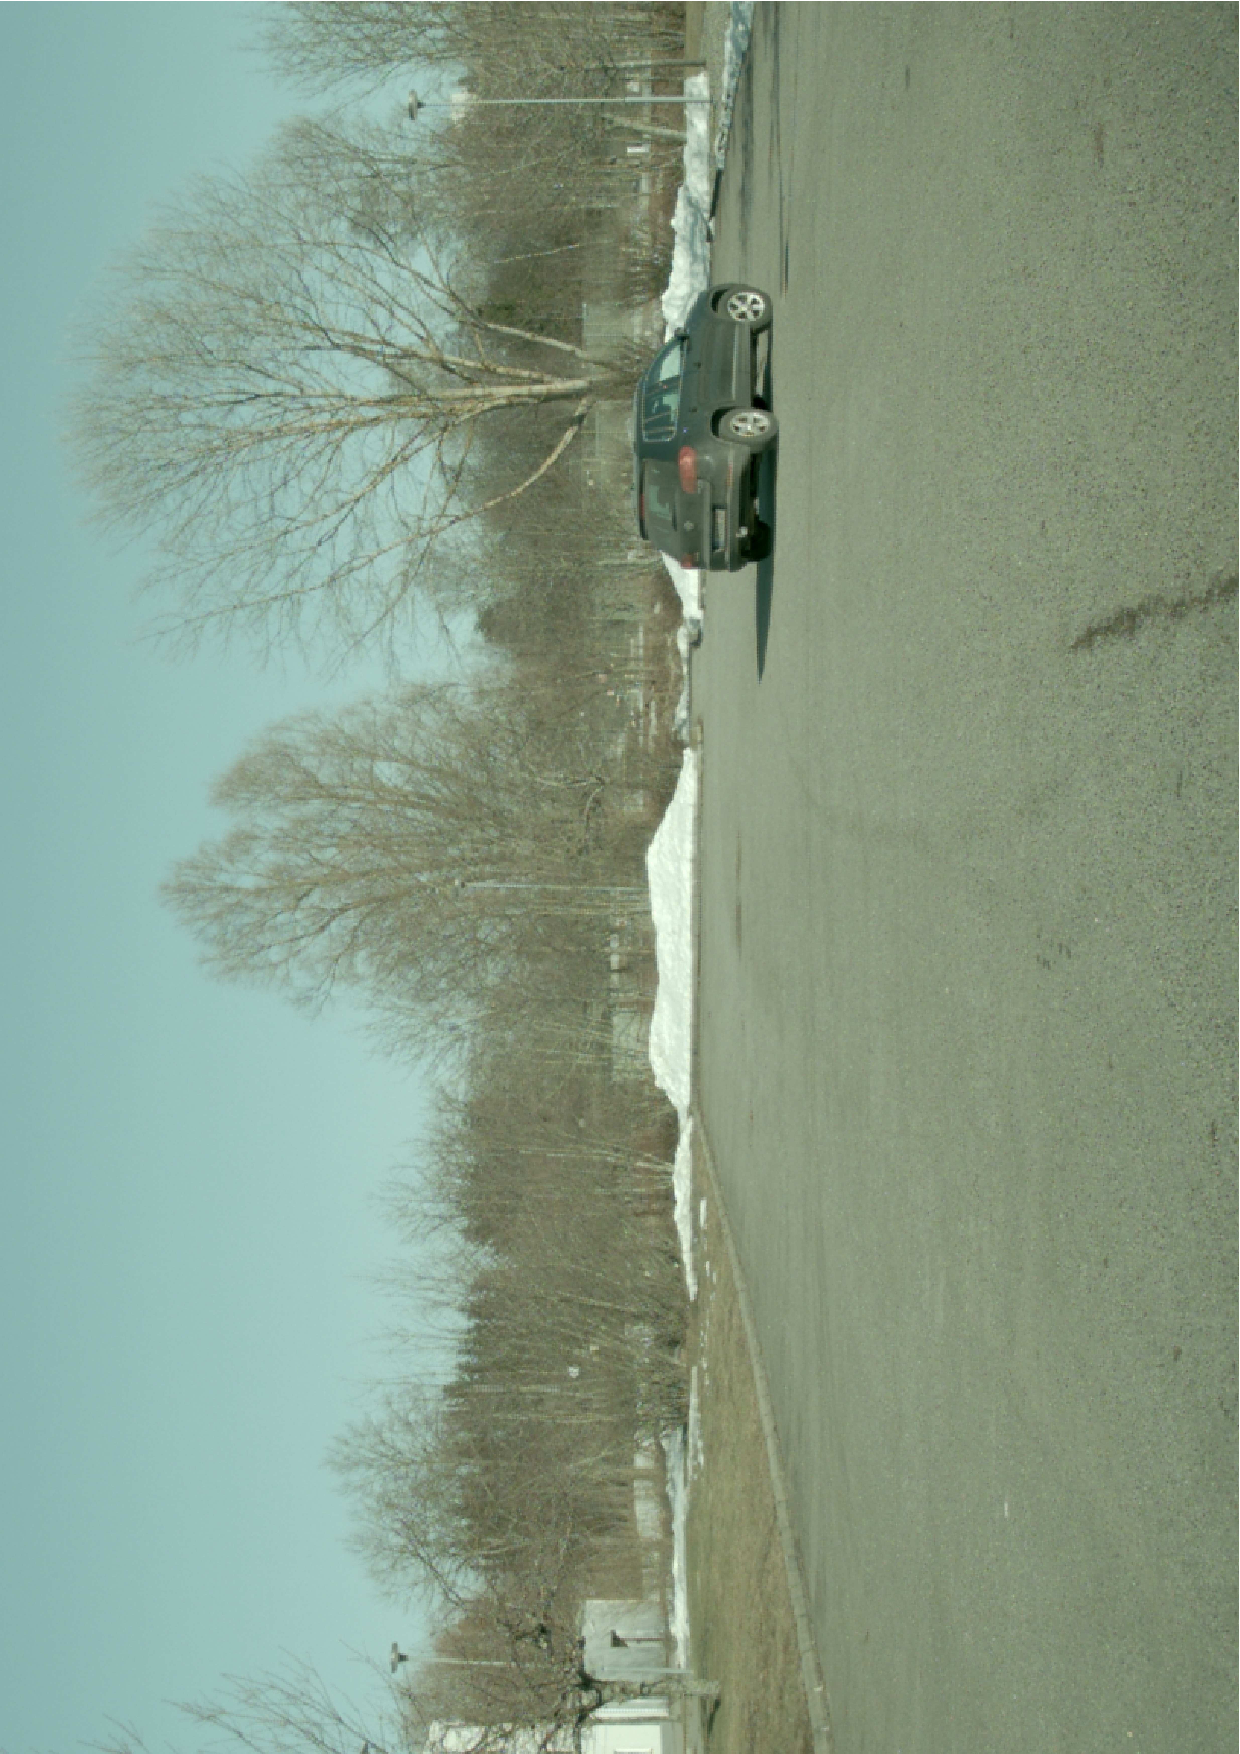
\includegraphics[angle=-90,origin=c,trim={0 0 5cm 0},width=0.55\textwidth]{Sequences/155733_95}
		\label{fig:155733_95}
	}
	\caption{\label{fig:sequence155733} The second sequence where the target vehicle drives straight and then turns to the right.}
\end{figure}

\begin{figure}[!ht]
	\centering
	\subfloat[][Comparison with a stereo camera system, using \abbrROI and angular rate as measurements in the mono camera system.]
	{
		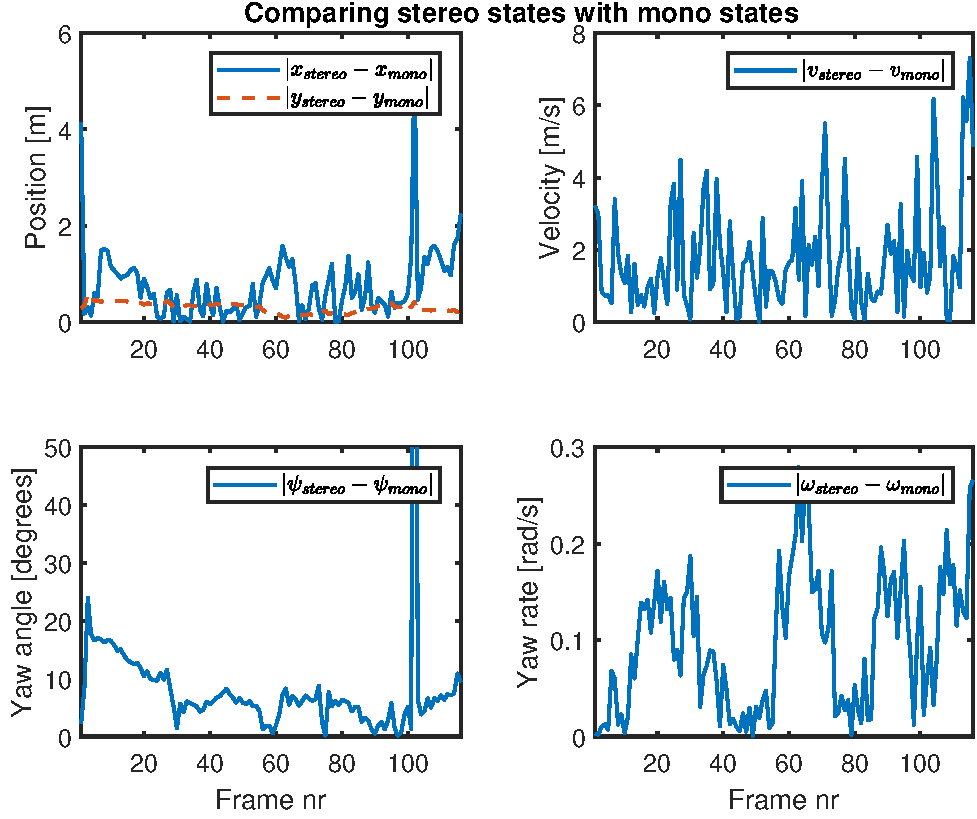
\includegraphics[width=0.7\textwidth]{StereoComparison/155532_RoiAngVel_gate_klt}
		\label{fig:roiangvel155532}
	}

	\subfloat[][Comparison with a stereo camera system, using \abbrROI and corners as measurements in the mono camera system.]
	{
		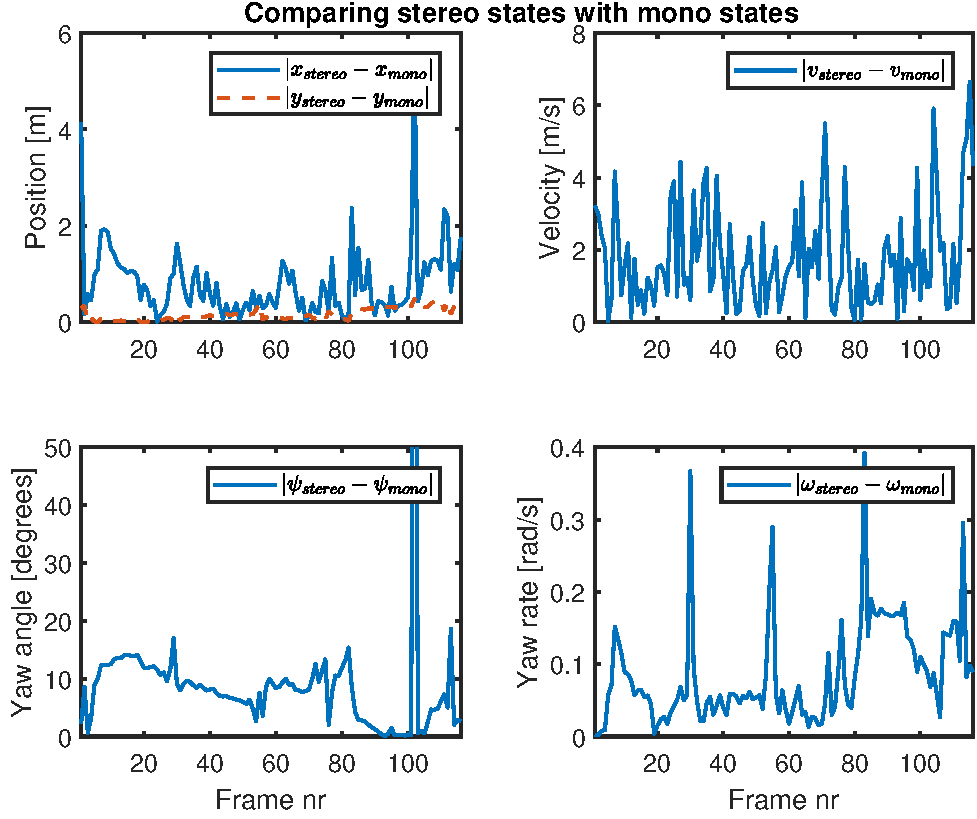
\includegraphics[width=0.7\textwidth]{StereoComparison/155532_RoiCorner_gate_klt}
		\label{fig:roicorner155532}
	}
	\caption{Comparison with a stereo camera system for the first sequence.}
\end{figure}

\begin{figure}[!ht]
	\centering
	\ContinuedFloat
	\subfloat[][Comparison with a stereo camera system, using all three measurements in the mono camera system.]
	{
		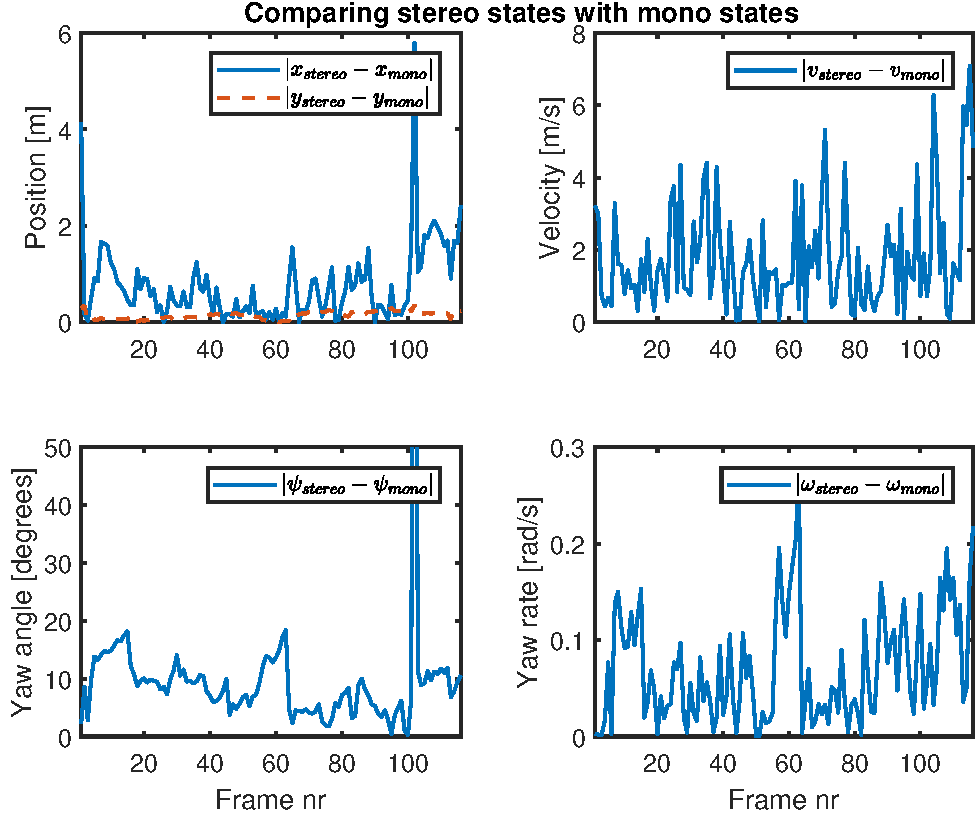
\includegraphics[width=0.7\textwidth]{StereoComparison/155532_AllMeasurements_gate_klt}
		\label{fig:all155532}
	}
	\caption{\label{fig:comparison155532} Comparison with a stereo camera system for the first sequence.}
\end{figure}

\begin{figure}[!ht]
	\centering
	\subfloat[][Comparison with a stereo camera system, using \abbrROI and angular rate as measurements in the mono camera system.]
	{
		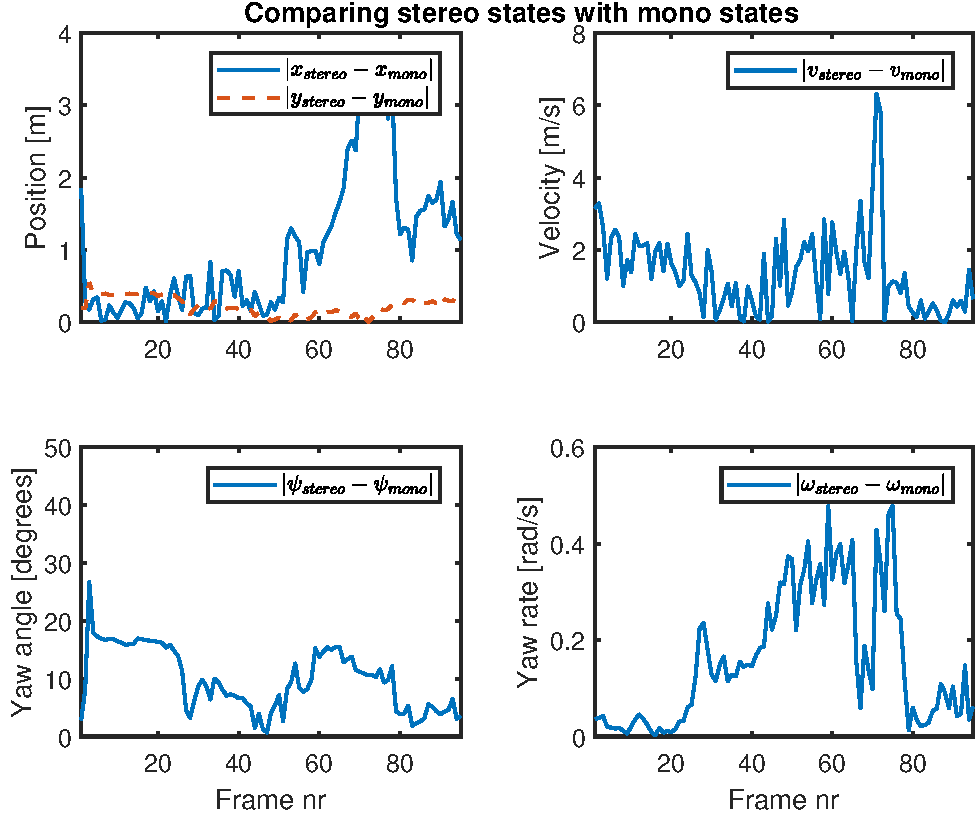
\includegraphics[width=0.7\textwidth]{StereoComparison/155733_RoiAngVel_gate_klt}
		\label{fig:roiangvel155733}
	}
	\caption{Comparison with a stereo camera system for the second sequence.}
\end{figure}

\begin{figure}[!ht]
	\centering
	\ContinuedFloat
	\subfloat[][Comparison with a stereo camera system, using \abbrROI and corners as measurements in the mono camera system.]
	{
		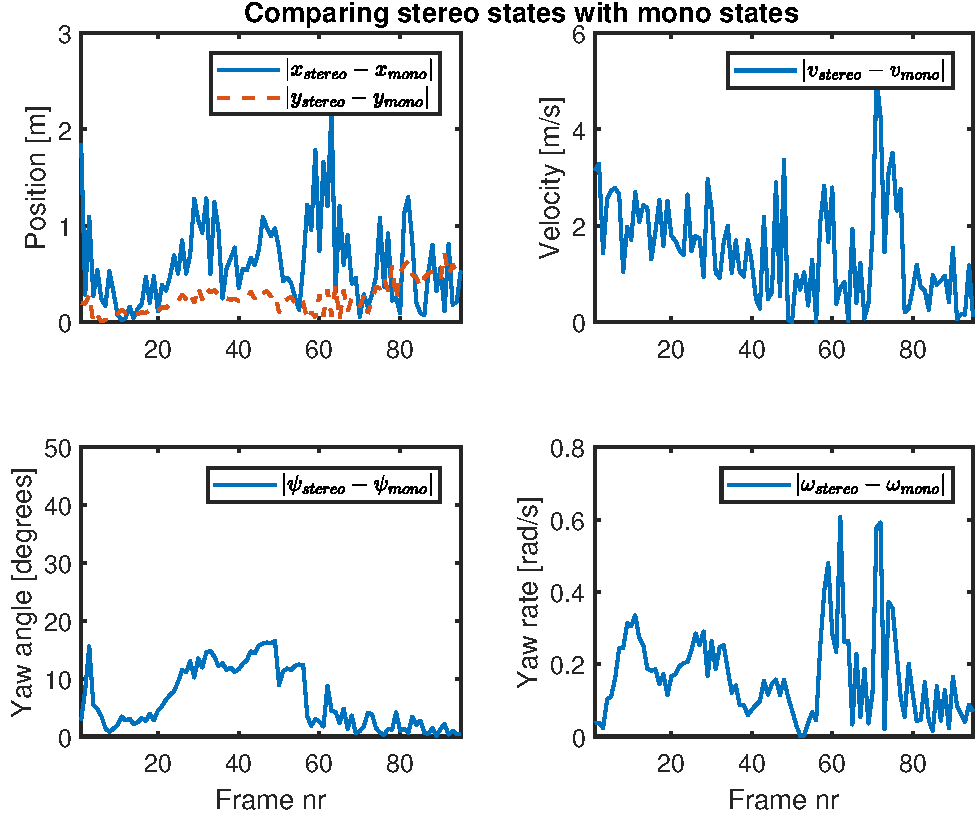
\includegraphics[width=0.7\textwidth]{StereoComparison/155733_RoiCorner_gate_klt_perf}
		\label{fig:roicorner155733}
	}

	\subfloat[][Comparison with a stereo camera system, using all three measurements in the mono camera system.]
	{
		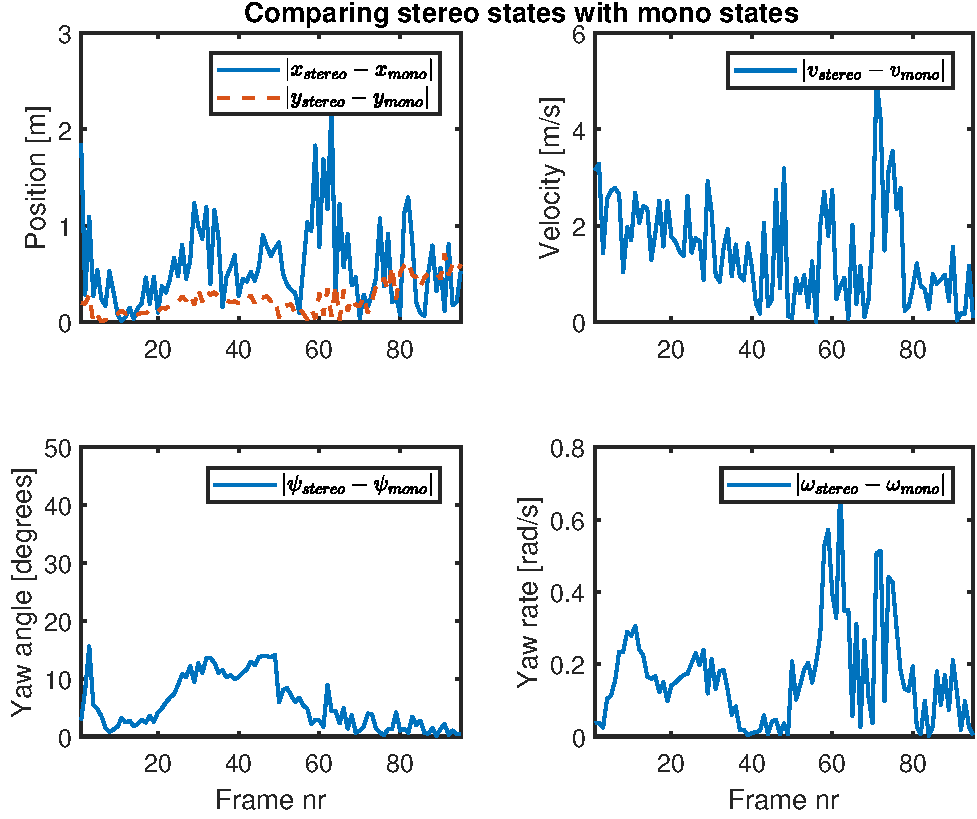
\includegraphics[width=0.7\textwidth]{StereoComparison/155733_AllMeasurements_gate_klt_perf}
		\label{fig:all155733}
	}
	\caption{\label{fig:comparison155733} Comparison with a stereo camera system for the second sequence.}
\end{figure}